\newpage
\section{评估NVIDIA新架构GPU的机器学习应用性能}
\setcounter{table}{0}
\setcounter{figure}{0}
\subsection{实验工具与环境}
\subsubsection{实验环境}
\par 表\ref{table-环境}中列出实验环境。\\
\begin{table}
	\centering
	\renewcommand{\thetable}{\arabic{section}-\arabic{table} }
	\renewcommand{\tablename}{表}
	\caption{实验环境}
	\addtocounter{table}{-1}
	\renewcommand{\thetable}{\arabic{section}-\arabic{table} }
	\renewcommand{\tablename}{Table}
	\caption{Environment}
	\begin{tabular}{cc}
		\toprule
		项目	&	内容\\
		\midrule
		CPU		&	AMD Ryzen ThreadRipper 2990WX 32C64T @ 3.0GHz\\
		主板		&	MSI X399\\
		内存		&	CORSAIR DDR4 3200 @ 16-15-15-15-34-1T 128GB\\
		GPU		&	NVIDIA Geforce RTX 2080TI (Turing)\\
		硬盘		&	INTEL750 NVMe PCIe 1.2TB * 2 @ RAID 0\\
		系统		&	Windows 10 64-bit build 17763\\	
		CUDA	&	10.1, 10.0, 9.2, 9.0\\
		其他		&	Jetson TX2 $ * $\\
		\bottomrule
		$ * $该硬件由NVIDIA提供。\\
	\end{tabular} 
	\label{table-环境}
\end{table}

\subsubsection{实验工具}
\par 实验中使用到了若干软件工具,如表\ref{table-实验工具}列出。
\begin{table}
	\centering
	\renewcommand{\thetable}{\arabic{section}-\arabic{table} }
	\renewcommand{\tablename}{表}
	\caption{实验工具}
	\addtocounter{table}{-1}
	\renewcommand{\thetable}{\arabic{section}-\arabic{table} }
	\renewcommand{\tablename}{Table}
	\caption{Tools}
	\begin{tabular}{cc}
		\toprule
		项目	&	内容\\
		\midrule
		Python 3.6		&	用于进行数据统计、编写TensorFlow应用\\
		Conda 4.5.12		&	用于创建、管理、隔离Python环境\\
		TensorFlow		&	1.12.0和1.13.0版本的源码,用于对比、研究、调整\\
		Bazel 0.16.0		&	用于从源码构建TensorFlow\\
		Msys2		&	用于从源码构建TensorFlow\\
		CMake 3.1.0		&	用于构建CUTLASS\\	
		Nsight 6.0	&	用于后台监听CUDA应用,捕捉Trace\\
		nvprof		&	用于分析CUDA程序的API调用、分支效率等\\
		git			&	版本控制\\
		Perforce	&	版本控制\\
		Ubuntu 16.04 Physical & 用于执行GPGPU-SIM 应用\\
		GPGPU-SIM 3.2 & 用于从指令级别模拟CUDA程序\\
		Visual Studio 2017 & 搭配10.0.17763.0版本的SDK\\
		\bottomrule
	\end{tabular} \label{table-实验工具} 
\end{table}
\subsection{实验详细过程}
\subsubsection{基于测试样例的Benchmark}
\par 为了为接下来的实验设定基准,这一步先使用用途单一的测试样例测试绝对性能以及相应的提升,因不同架构的硬件各项参数(包括流处理器数量、显存容量等)不尽相同,所以直接对比不同架构硬件的性能是没有意义的,这里选择对比不同架构硬件在不同SDK下性能提升的比例。此处选用了CUDA 10.0,CUDA 9.2,CUDA 9.0三种SDK,同时选用9.2与9.0的原因是因为9.2版本是为了图灵架构的GPU Tesla V100发布的\parencite{CUDA92},也在本文的研究范围内。
\par 因为本文主要讨论新架构GPU在机器学习应用中带来的性能提升,故选用的评测样例大部分都与机器学习应用相关;主要从以下角度进行评估:通用矩阵乘法(GEMM, General Matrix Multiply)、矩阵乘法运算性能、卷积运算性能、神经网络推理性能以及结合框架的综合性能。在评估这些性能时也会包含单/双精度浮点计算性能。
\paragraph{通用矩阵乘法(GEMM, General Matrix Multiply)}
\par 作为新硬件最为鲜明的特点,本节将对张量核心以及相应的通用矩阵乘法运算进行评估,通用矩阵乘法运算又被称为混合矩阵运算,其混合体现在:运算中同时有加法和乘法,且精度同时涉及半精度浮点、单精度浮点和8位整数。与矩阵乘法相比,通用矩阵乘法被定义为:
$$ C \leftarrow \alpha AB + \beta C $$
\par 若将$ \beta $置为0,则该运算变为矩阵乘法运算。通用矩阵乘法这一运算在神经网络训练、推理中十分常见,根据官方文档,目前张量核心仅能用在CNN/RNN等特定结构的神经网络上,且只能用于前馈和反馈两部分。这个范围看起来很宅,然而在深度学习中占到了非常高的比重。式中操作数分别代表输入、权重和偏置,下文将简写为矩阵乘加。NVIDIA在新的伏特架构与图灵架构中加入的张量核心(Tensor Core)正是专门加速这种运算的硬件。
\subparagraph{实验结果}
\par 根据开发者社区的反映,新架构硬件性能的差别主要体现在问题规模、问题类型等方面(张量维度、形状,训练/推理任务等),而NVIDIA官方仅给出一种规模的结果,所以本节使用了自行编写的一系列测试用例,辅以深度学习测试套件DeepBench\parencite{DEEPBENCH},在开启和关闭新架构中张量核心的情况下进行测试。实验性能使用TFlops/s统计,方法为简单的运算数除以运算时间,运算时间的统计采用CUDA内置的$ cudaEvent $记录。
\par 首先评估的是在不同问题规模下,开启和关闭新架构中的张量核心所能达到的性能,如图\ref{Fig-PerfGemm}所示。随着问题规模的上升,总体加速比呈上升趋势,在大规模数据时半精度通用矩阵运算性能的加速比能达到3到3.5倍、单精度通用矩阵运算性能的加速比能达到2倍。然而,单纯考察数据规模发现加速比差距非常大,甚至是在大规模数据中仍然存在开启张量核心后性能不如不开启张量核心的情况,结合文档在通用矩阵运算一章中在指令中需要指明运算的最小单元这一点中\parencite{PTX};可以推测出输入矩阵的“形状”对张量核心的性能由较大影响。
\par 为了研究输入矩阵“形状”对于加速比的影响,由于两个输入矩阵涉及三个维度,故采用控制变量法,控制$ m,n,k $中某一维度考察另外两个维度对于加速比的影响。由于测试数据中存在部分离群值($ N\geq 500000 $),这会对作图精度产生极大影响,故先予以剔除。实验结果如图\ref{Fig-MNKRatio}所示。可见在两个输入矩阵的三个维度中,两矩阵共享的维度$ K $对于性能的影响最为显著。
\par 关于矩阵的形状、维度对于性能的影响,其原因将在后文结果分析中详细说明。以上实验数据以及性能旨在考查开启和关闭张量核心时性能提升幅度,故开启的线程块数量和线程数量较小,相应的GPU占用率也较小,导致所得性能并非GPU峰值性能。为测量峰值性能,这里还是用NVIDIA官方发布的用于线性代数计算的模板库CUTLASS(CUDA Template Linear Algebra Subroutines),该模板库根据新架构硬件特性编写,提供了许多测试样例供参考,这里使用CUTLASS测试得到的性能作为峰值性能基准。
\par CUTLASS库中的GEMM运算有多种精度可供选择:HGEMM、SGEMM、DGEMM、CGEMM、ZGEMM和IGEMM,分别代表半精度浮点、单精度浮点、双精度浮点、单精度复数、双精度复数和八位整数。鉴于之前的测试并不涉及复数,此处也不选用复数精度作为基准。需要注意的是测试样例后缀中存在$ \_[n/t][n/t] $分别代表运算中输入矩阵的数据存储、分布方式,即行列是否转置(如上文提到的,CUDA中矩阵存储分行主元素和列主元素存储)。图\ref{Fig-GEMM-CUTLASS}为测得的性能基准。
\begin{figure}
	\centering
	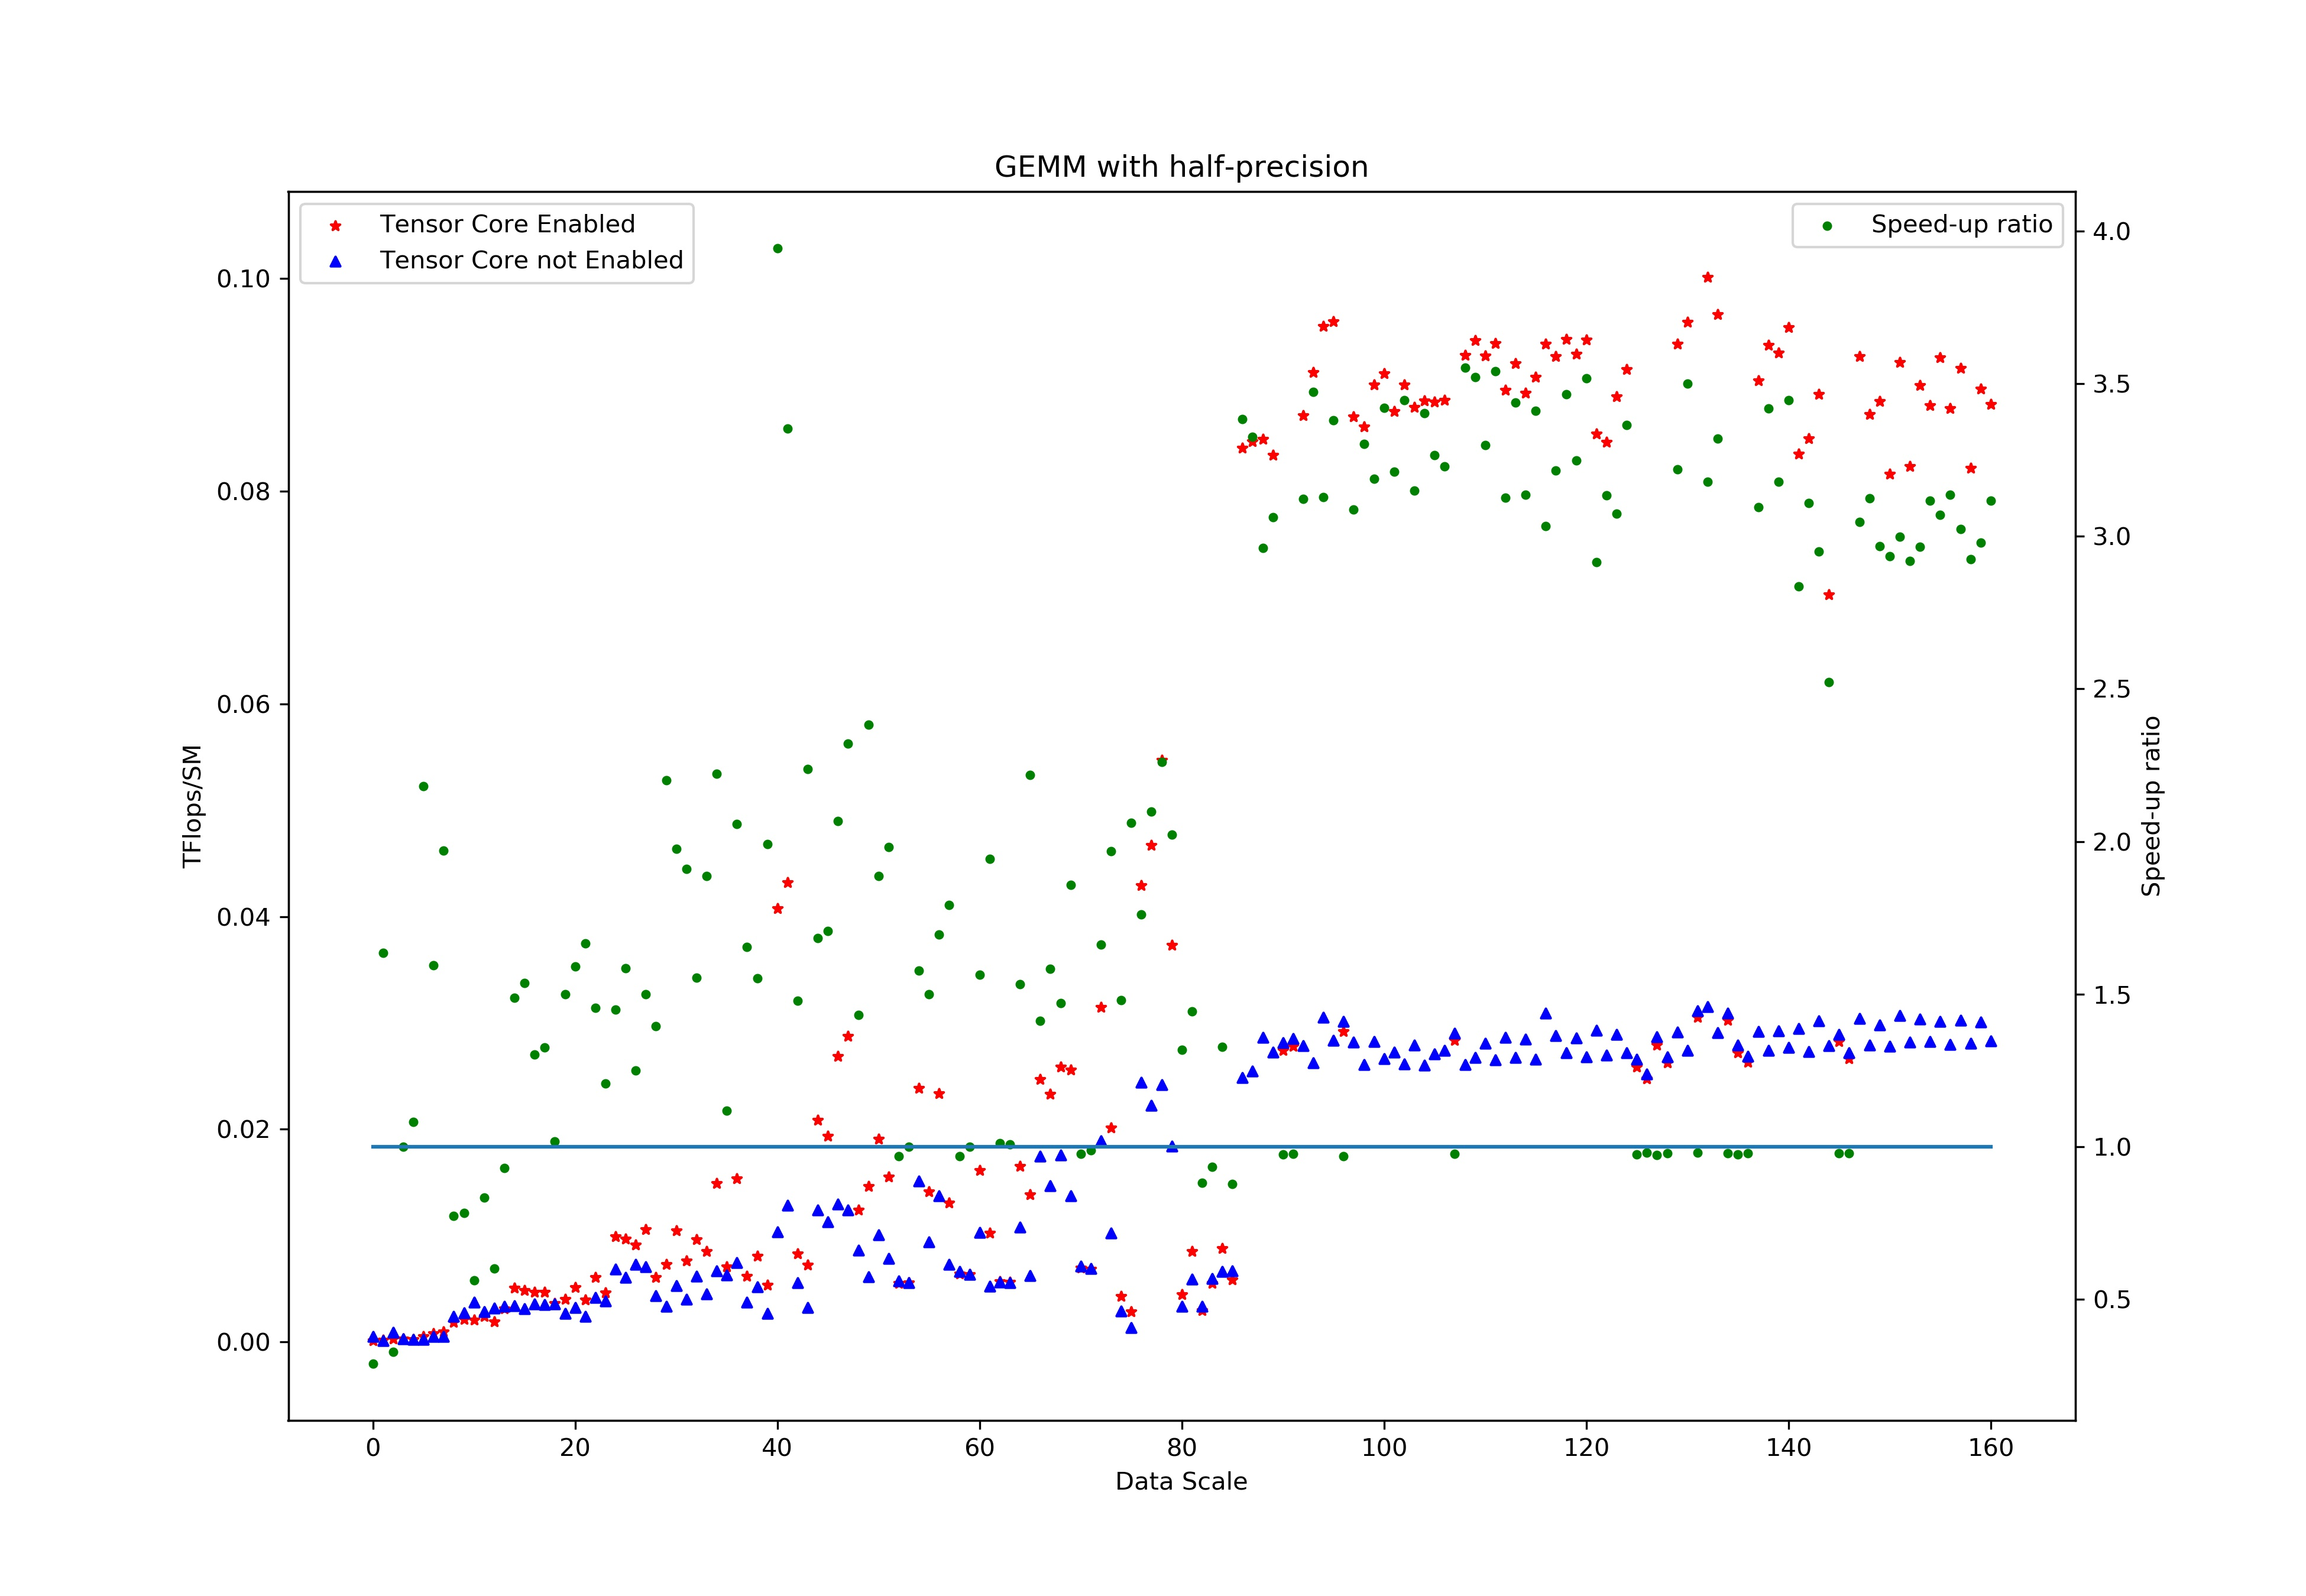
\includegraphics[width=7.5cm]{figures/GEMM-Half-TF.jpg}
	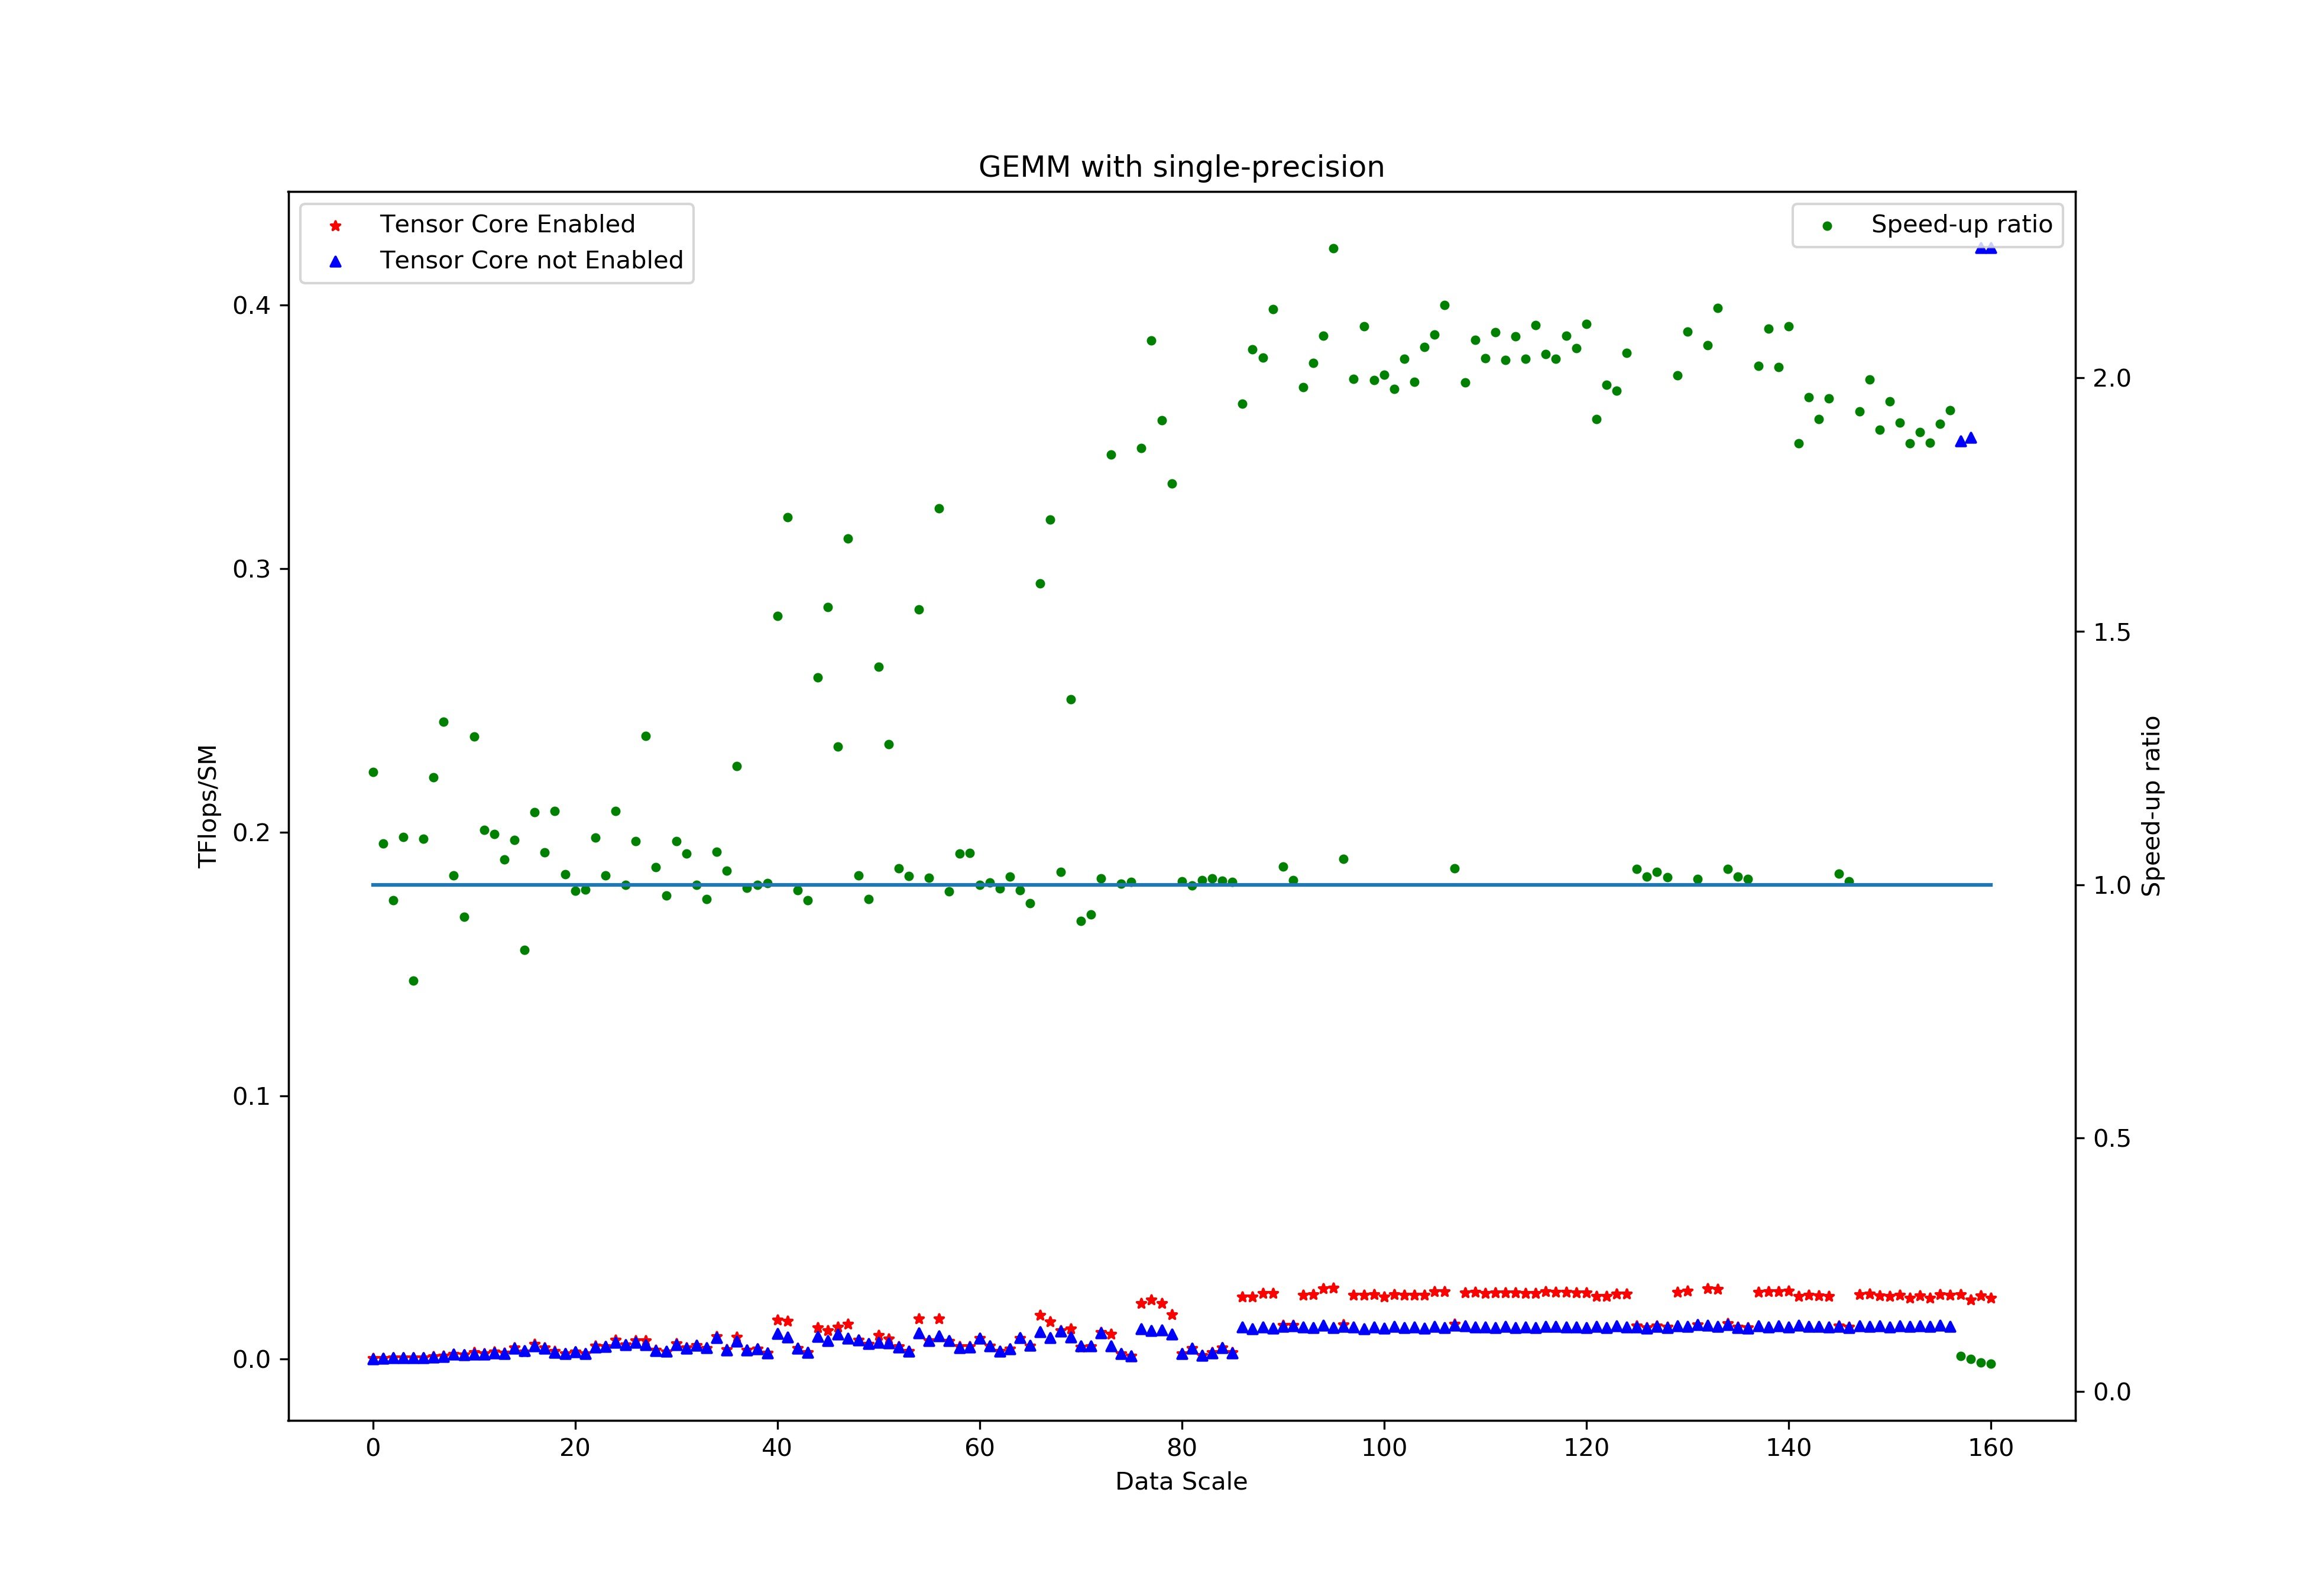
\includegraphics[width=7.5cm]{figures/GEMM-Single-TF.jpg}
	\renewcommand{\thefigure}{\arabic{section}-\arabic{figure} }
	\renewcommand{\figurename}{图}
	\caption{半精度/单精度GEMM性能}
	\addtocounter{figure}{-1}
	\renewcommand{\thefigure}{\arabic{section}-\arabic{figure} }
	\renewcommand{\figurename}{Figure}
	\caption{Performance of GEMM at Half and Single}
	\label{Fig-PerfGemm}
\end{figure}
\begin{figure}
	\centering
	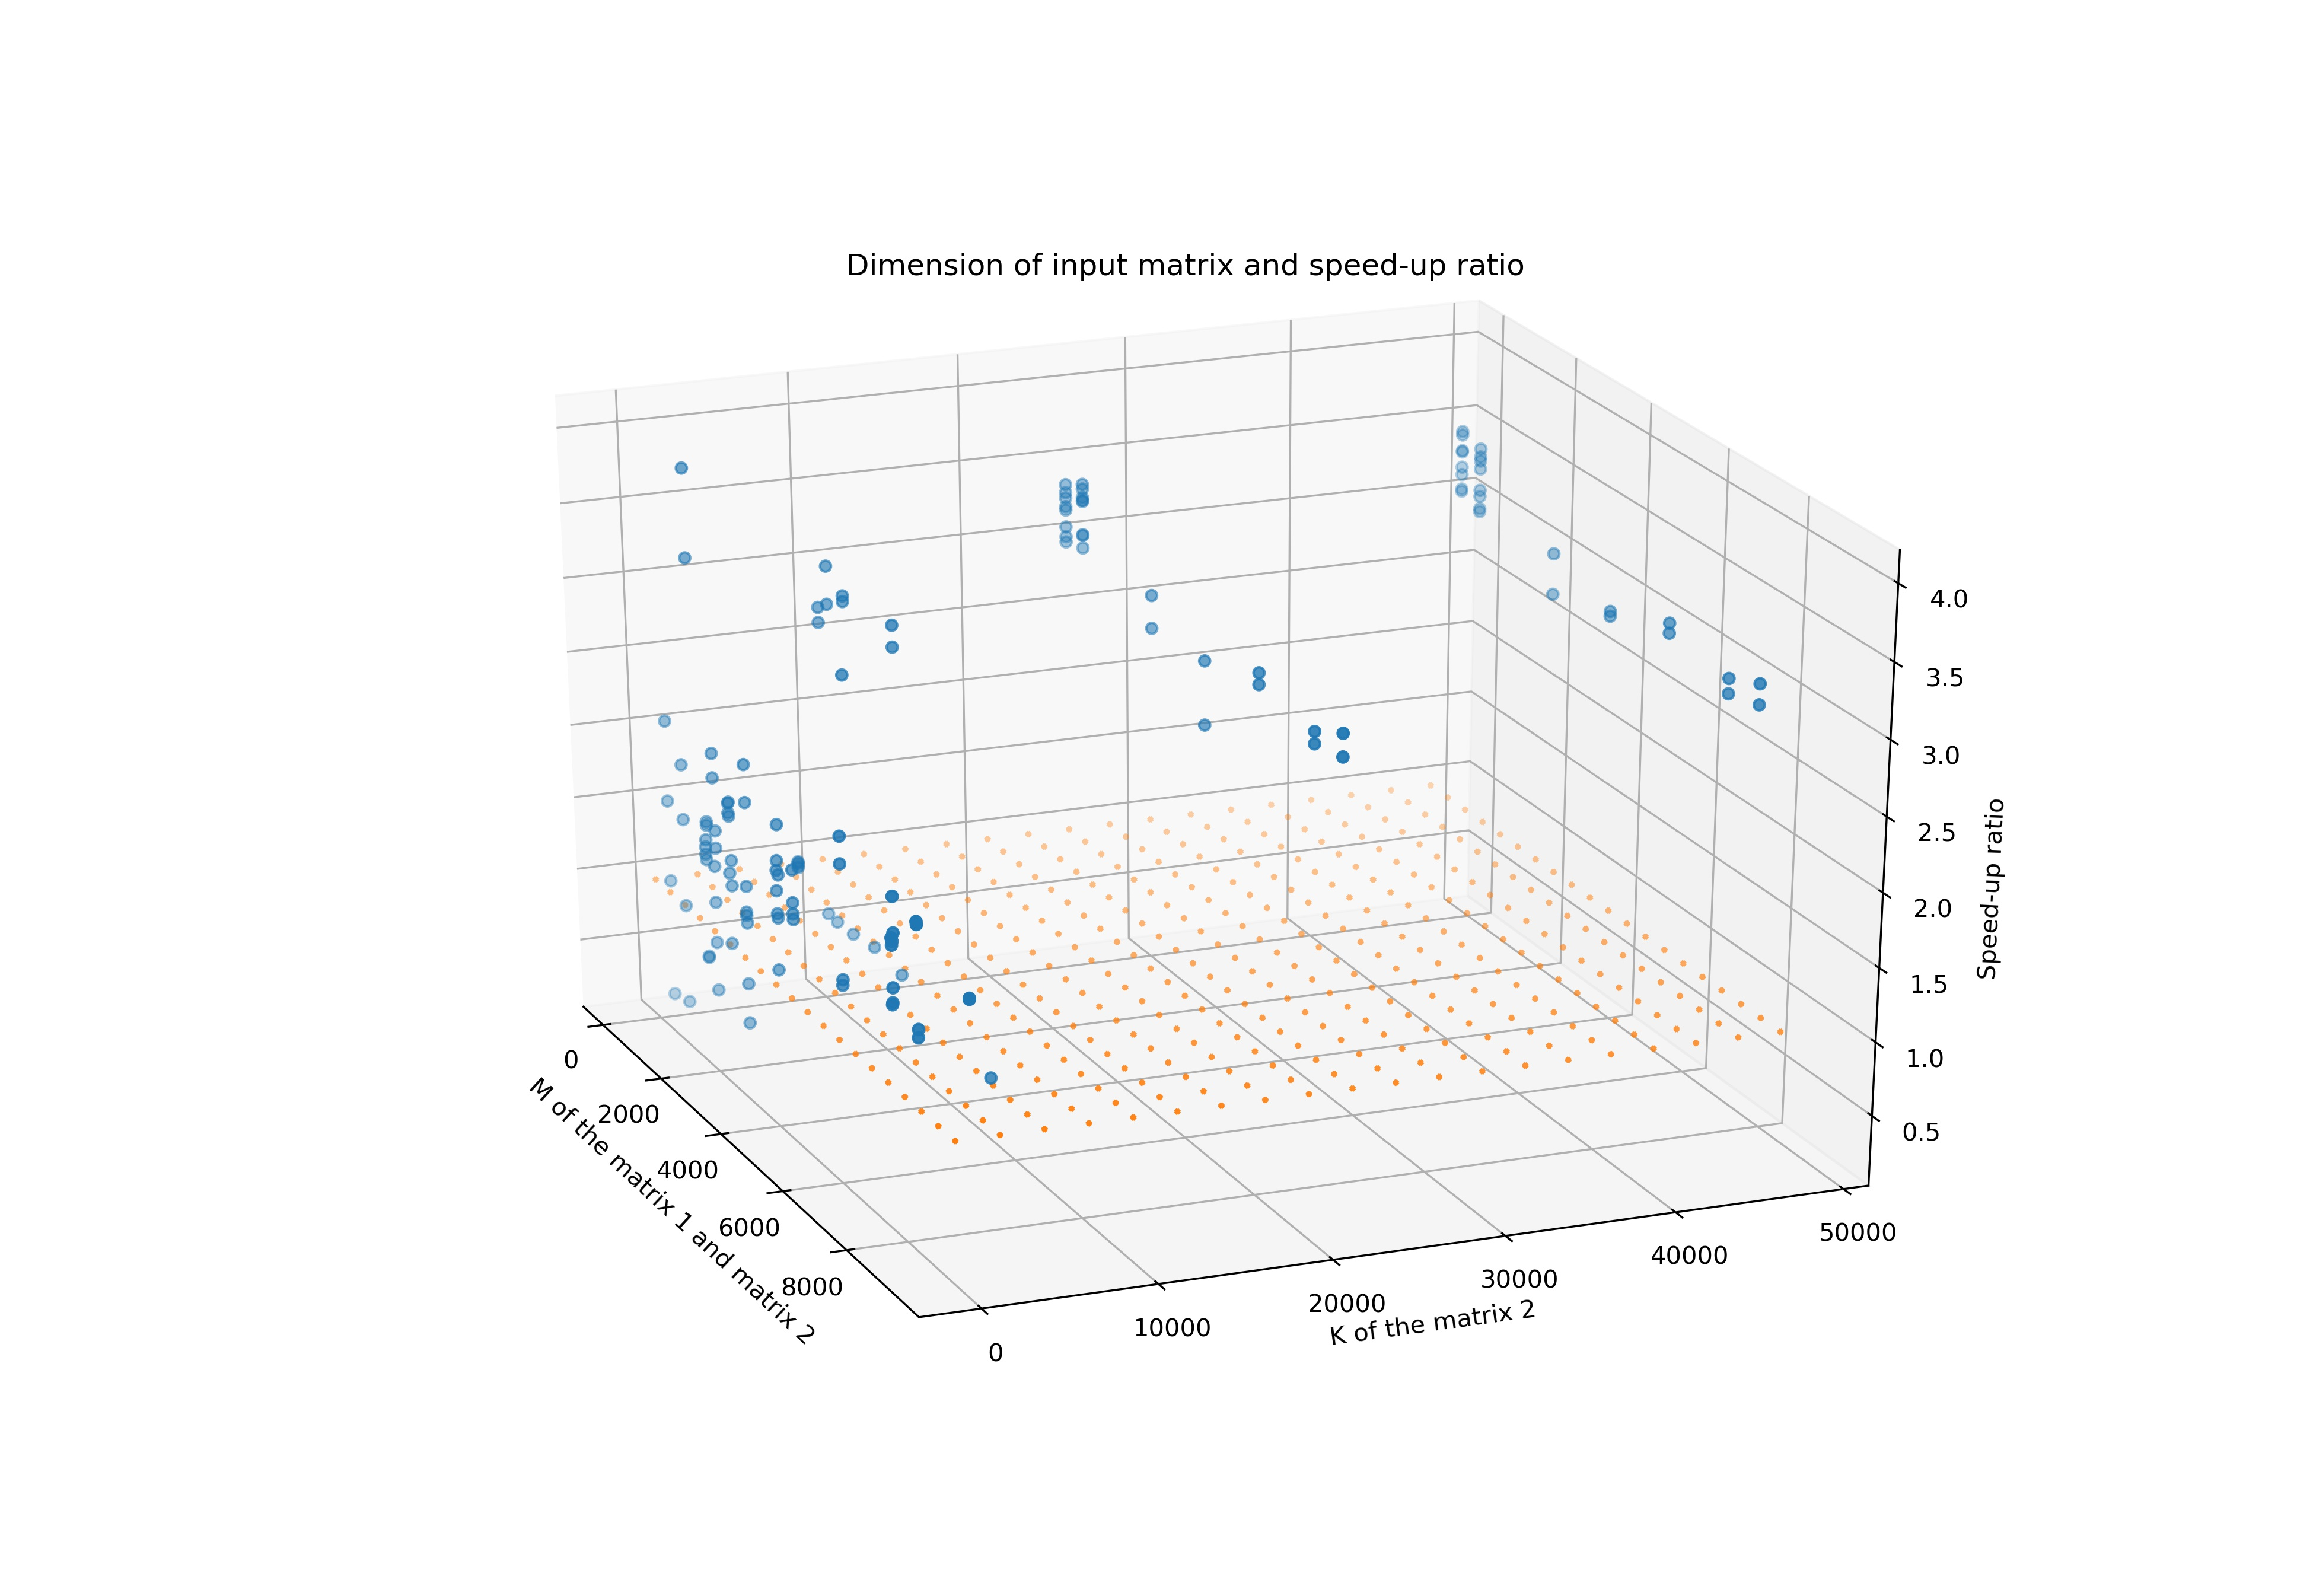
\includegraphics[width=7.5cm]{figures/GEMM_MK.jpg}
	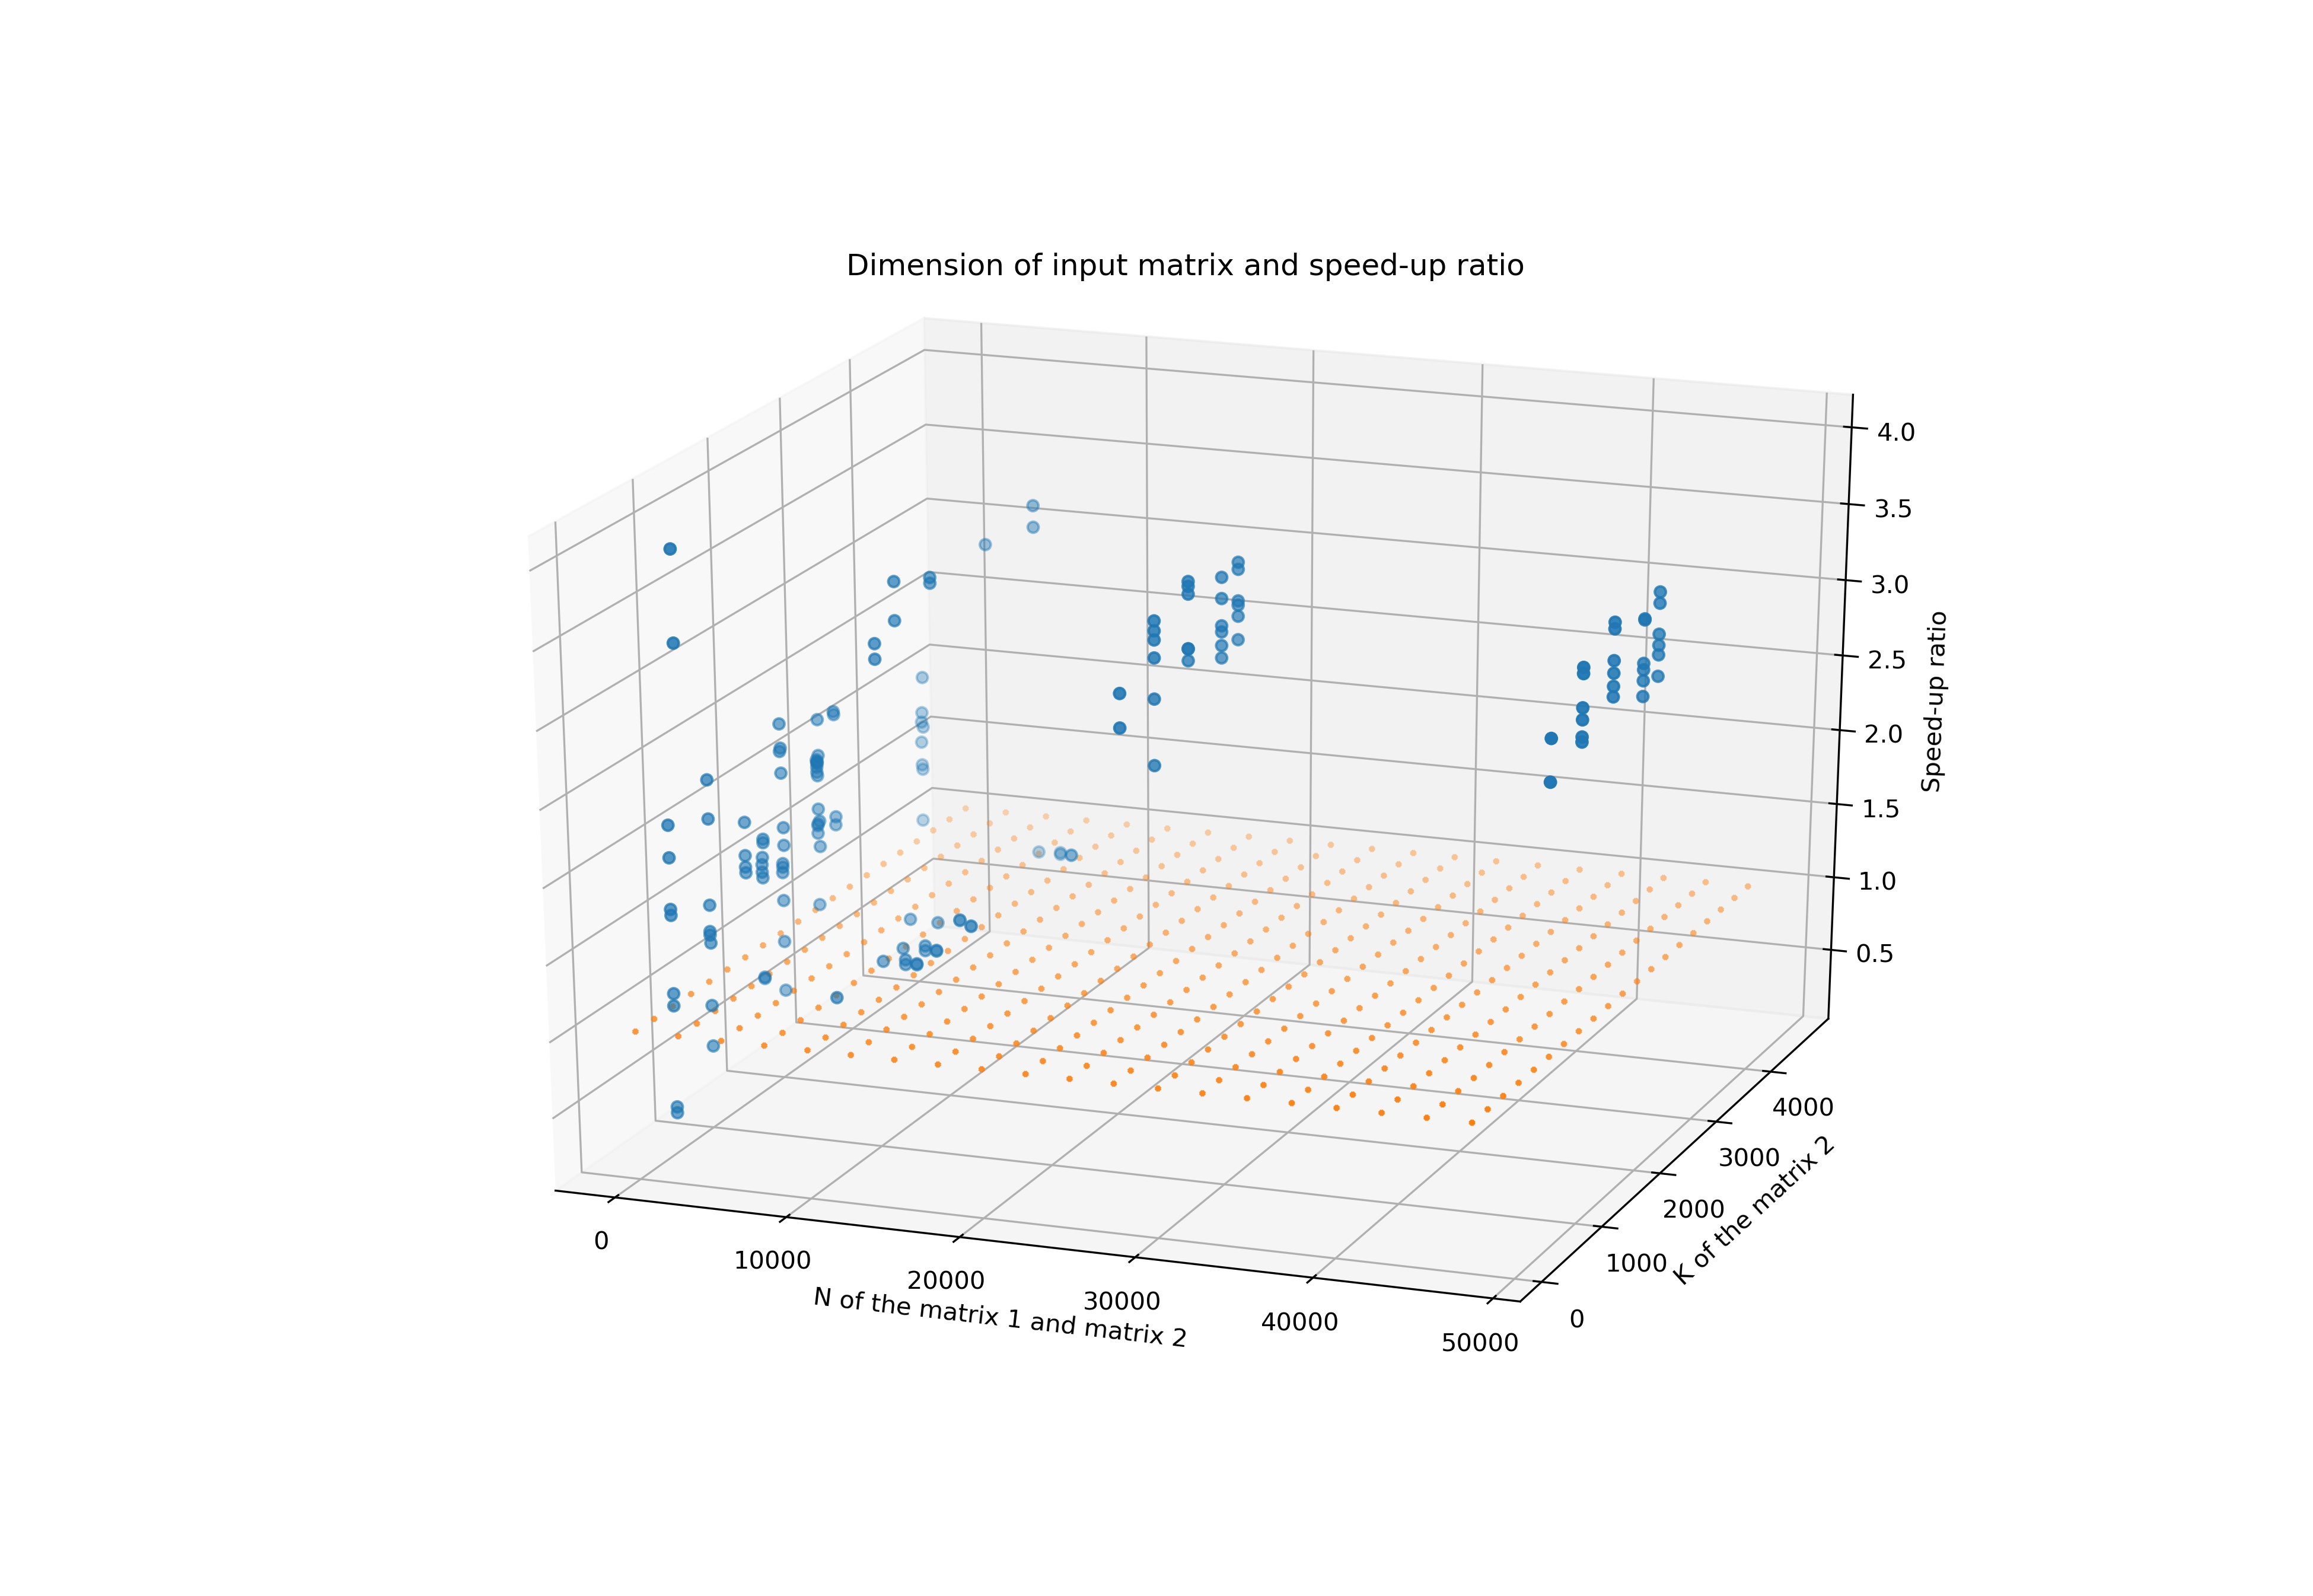
\includegraphics[width=7.5cm]{figures/GEMM_NK.jpg}\\
	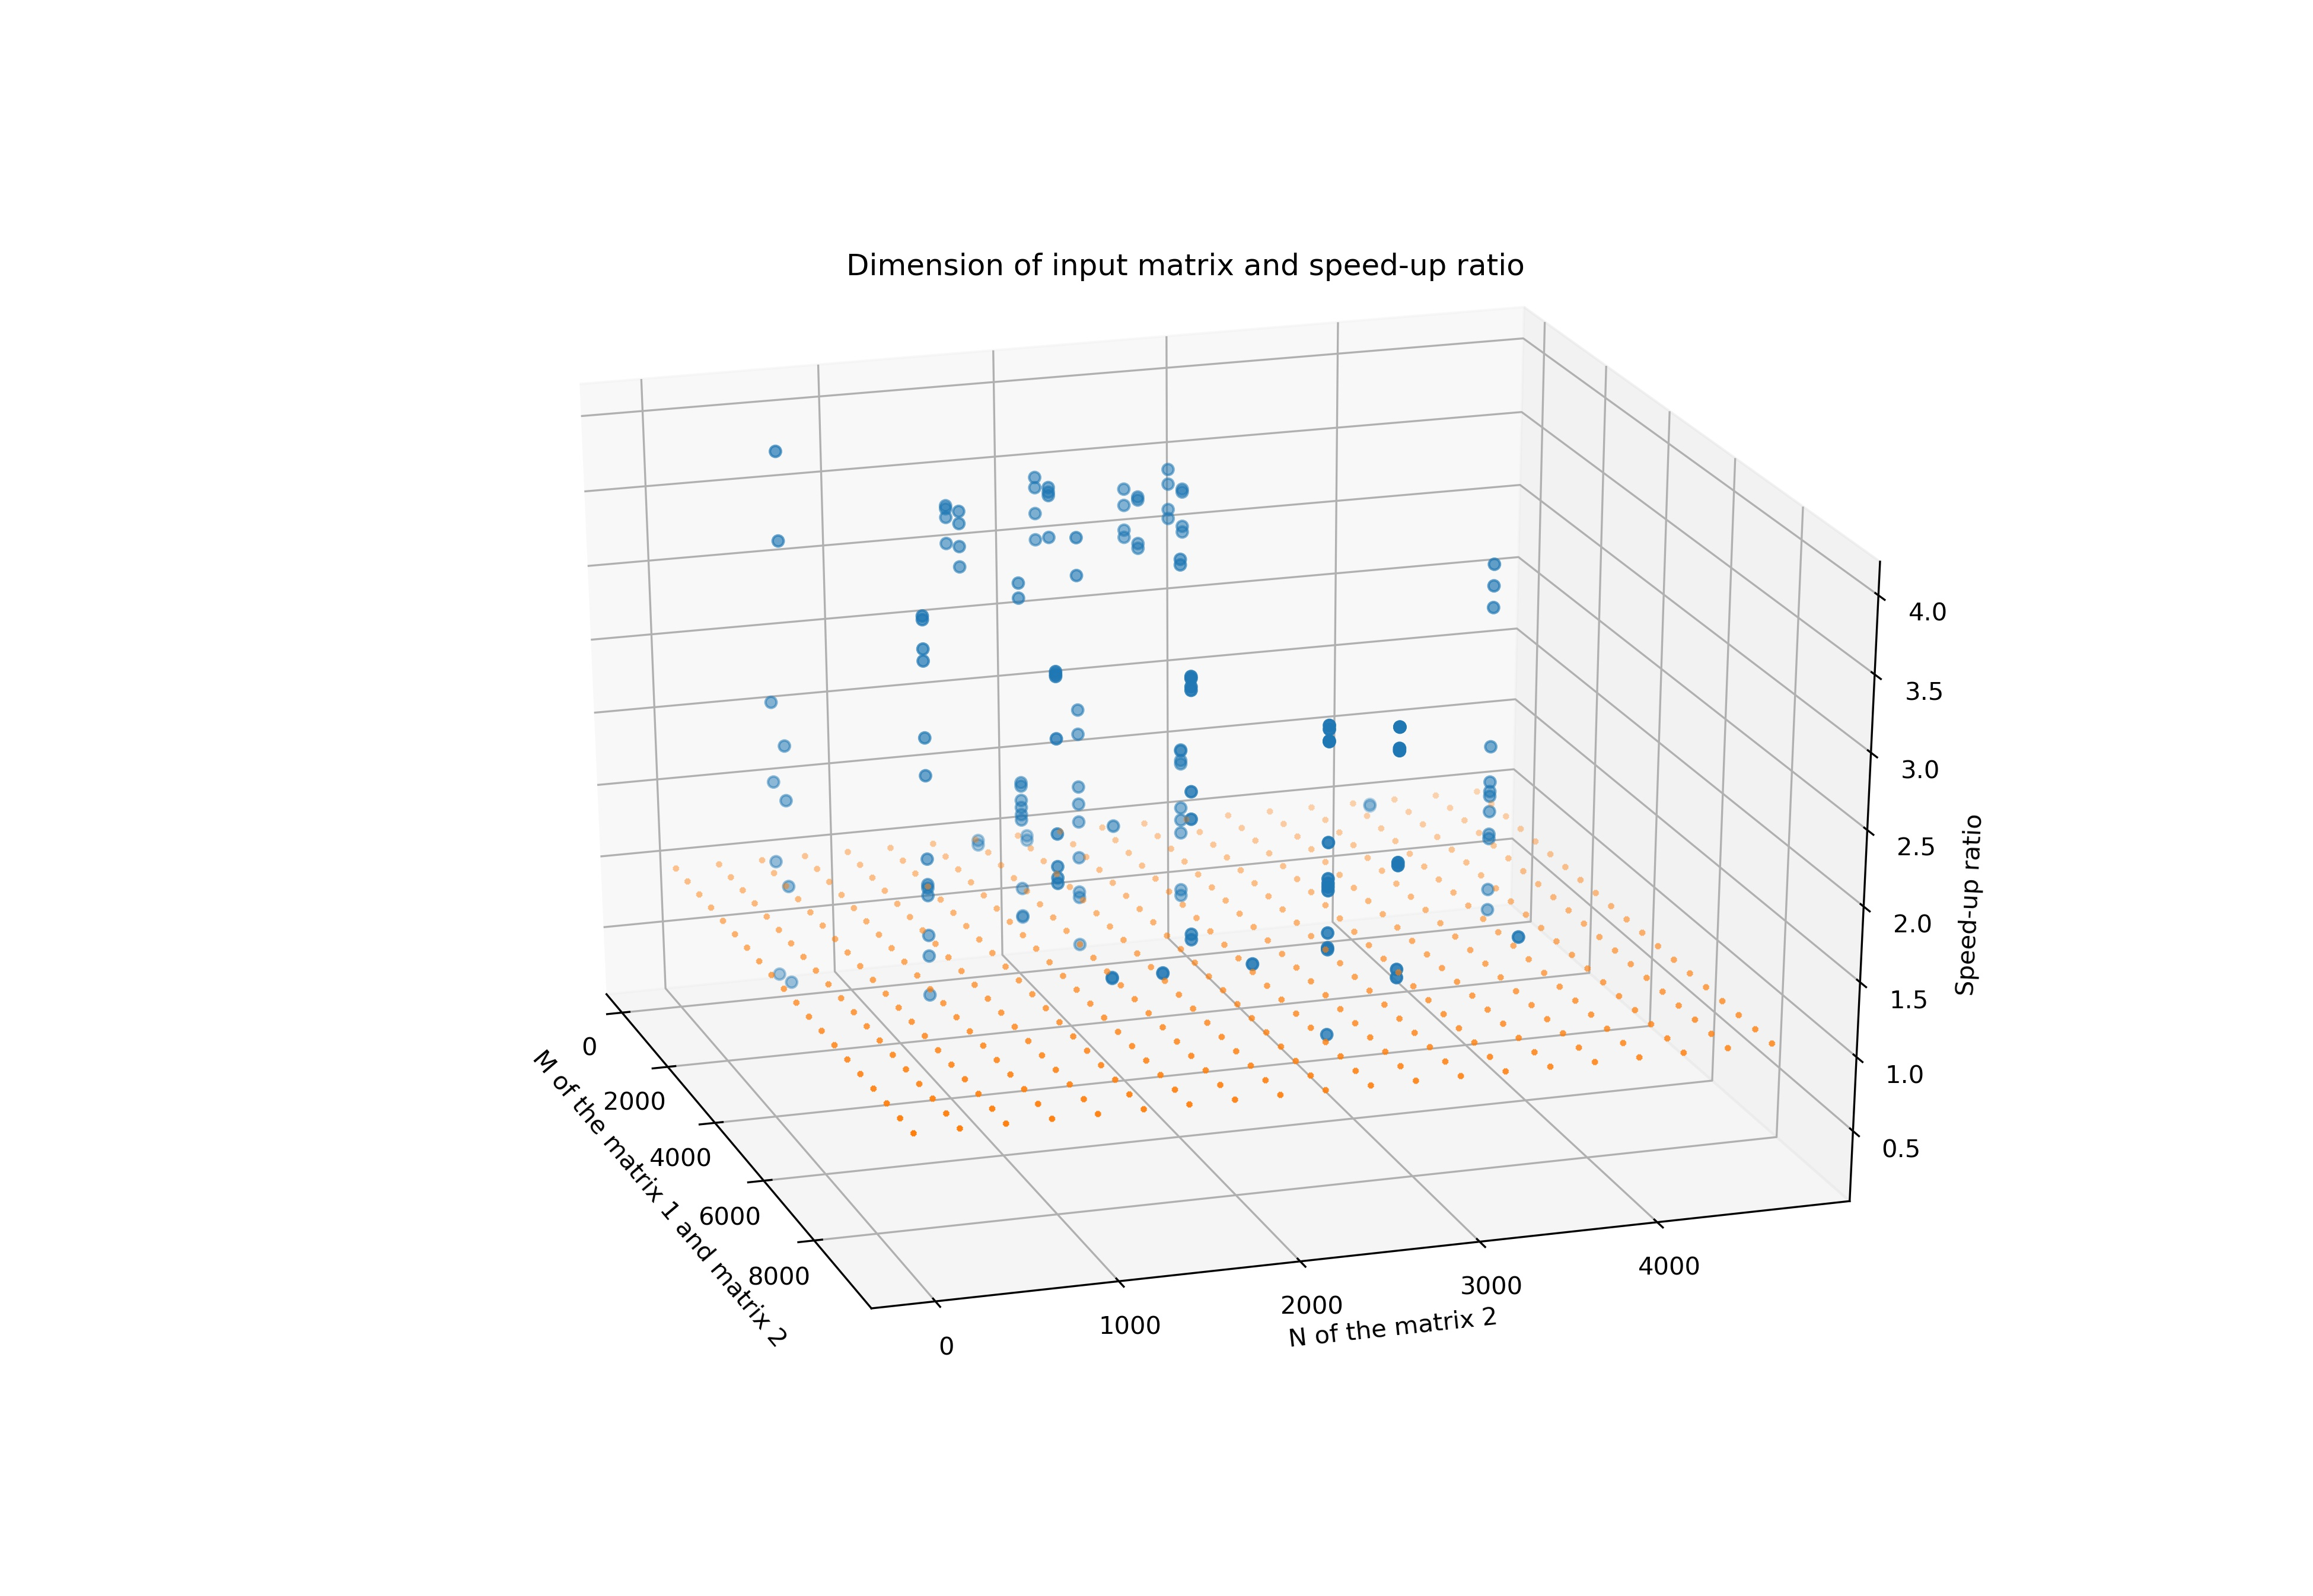
\includegraphics[width=7.5cm]{figures/GEMM_MN.jpg}
	\renewcommand{\thefigure}{\arabic{section}-\arabic{figure} }
	\renewcommand{\figurename}{图}
	\caption{输入矩阵维度与加速比的关系}
	\addtocounter{figure}{-1}
	\renewcommand{\thefigure}{\arabic{section}-\arabic{figure} }
	\renewcommand{\figurename}{Figure}
	\caption{Relationship of input matrix dimension and speed-up ratio}
	\label{Fig-MNKRatio}
\end{figure}
\begin{figure}
	\centering
	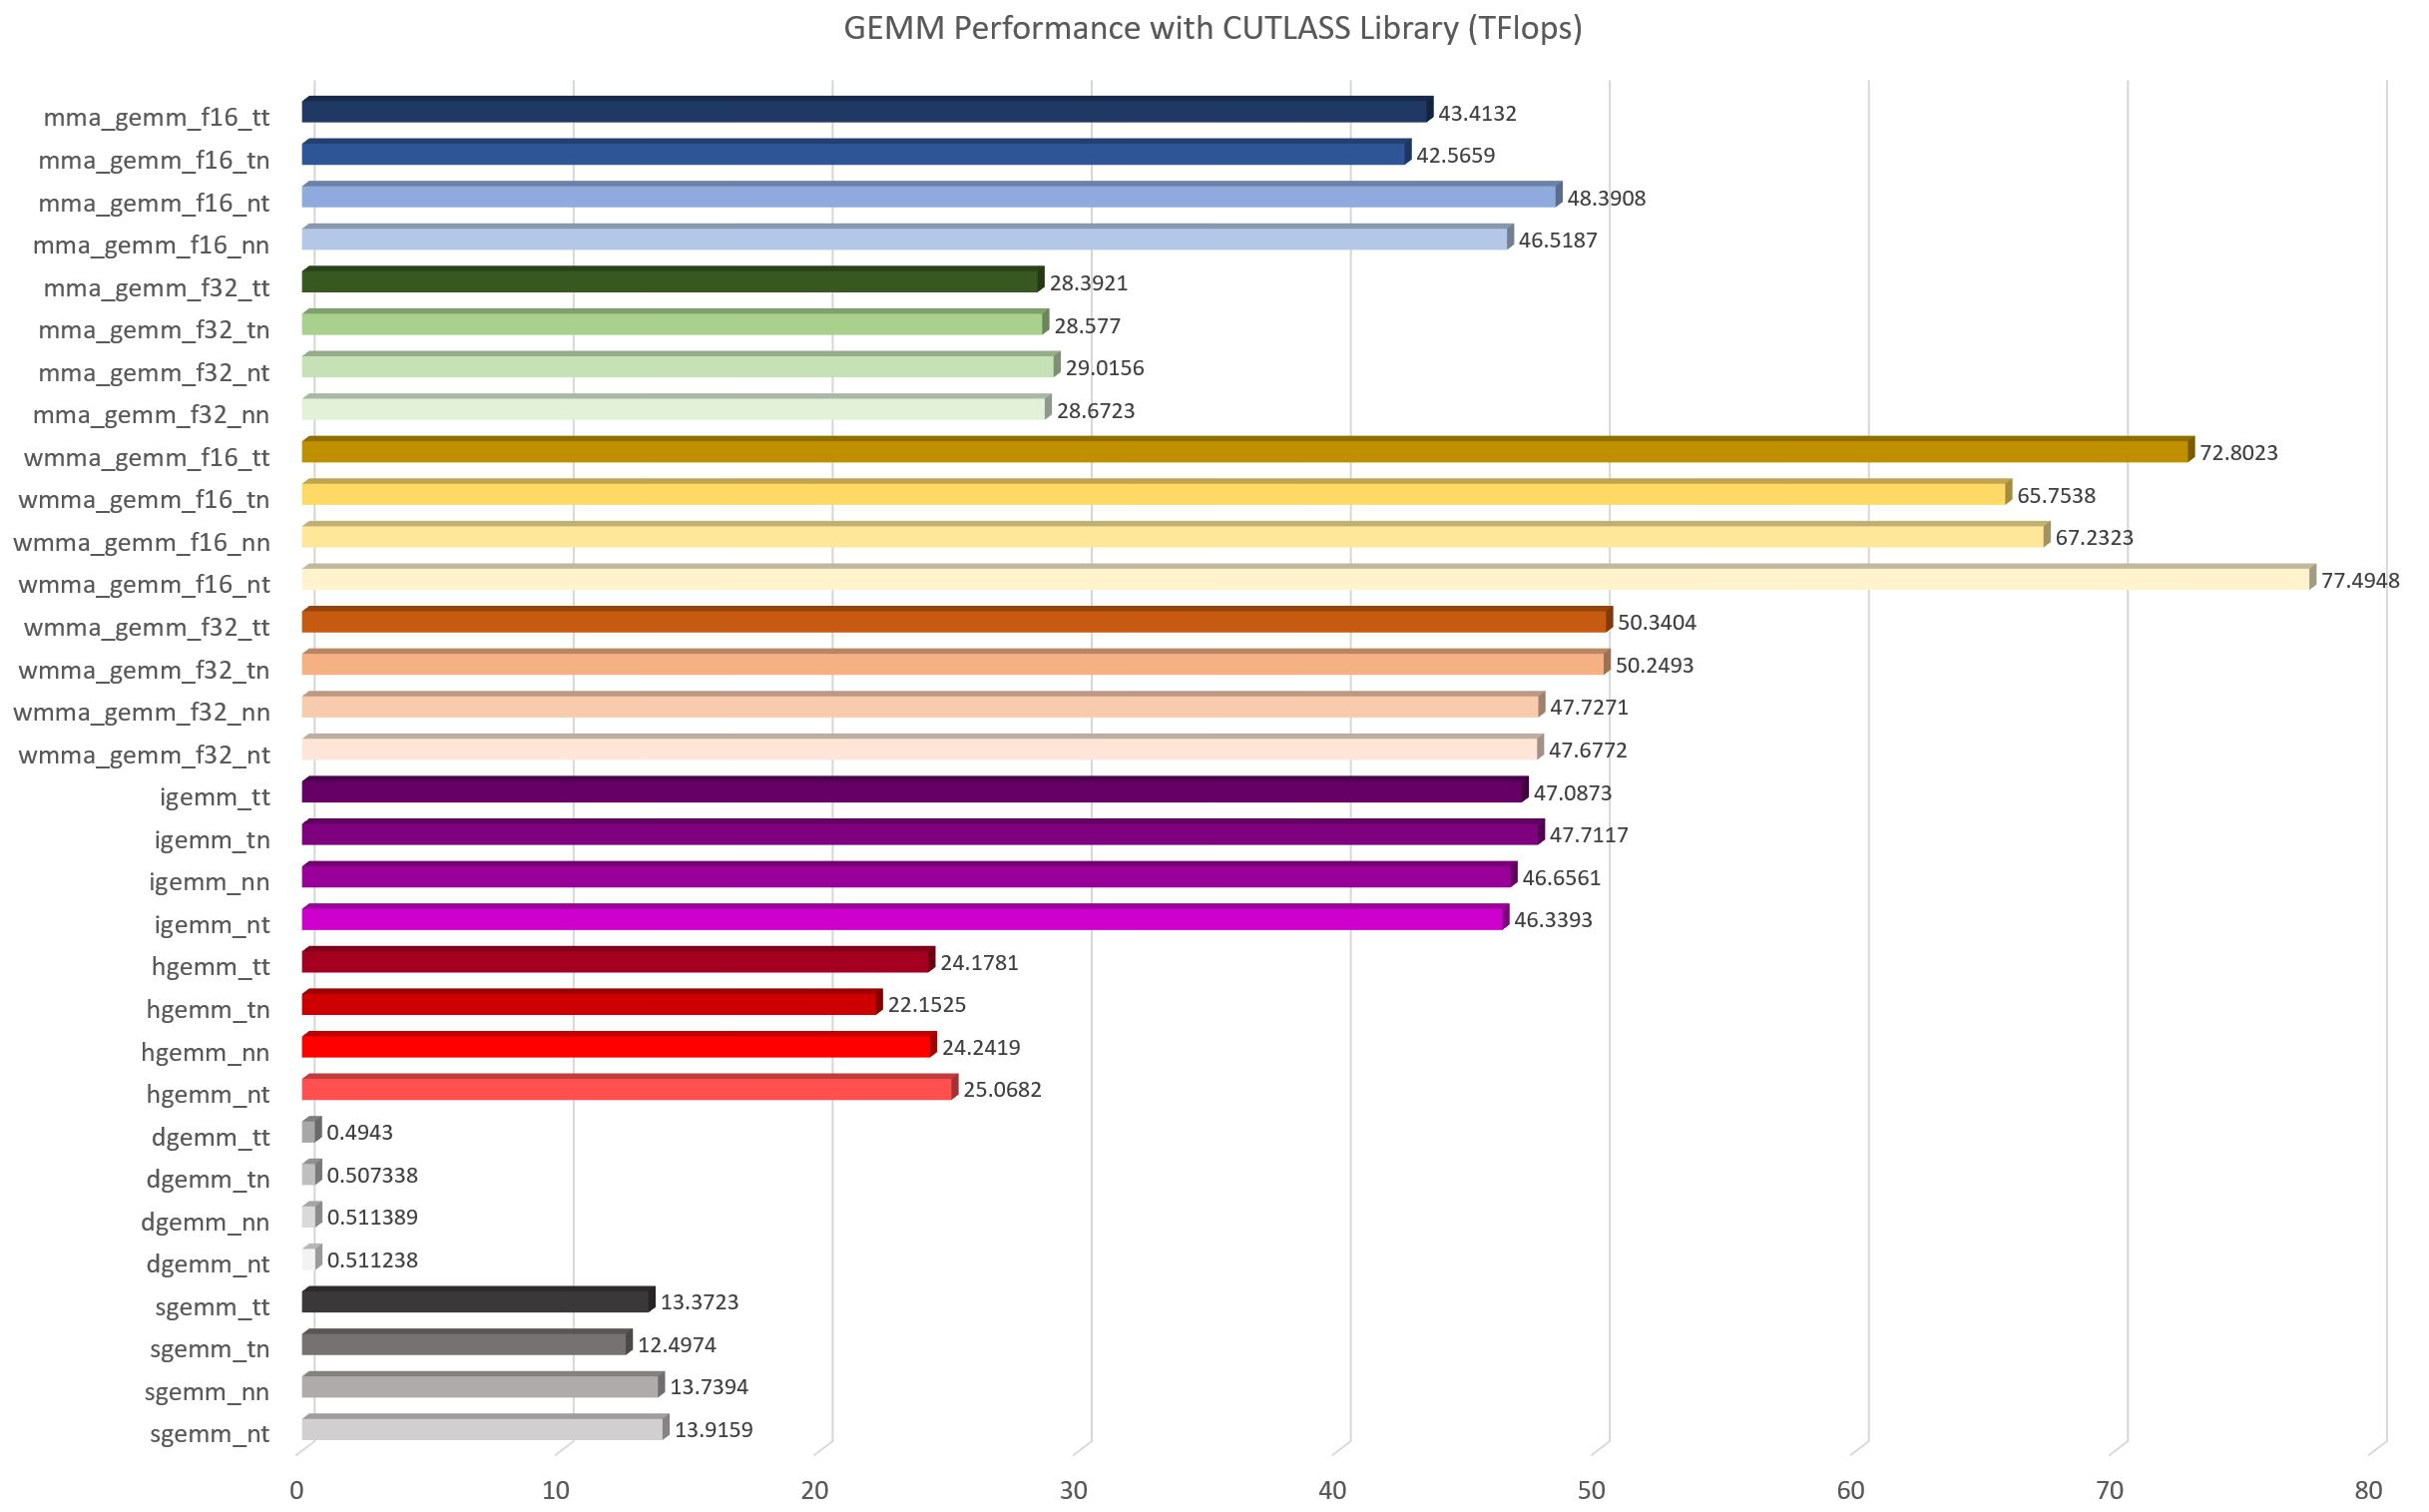
\includegraphics[width=15cm]{figures/CUTLASSGEMM.jpg}
	\renewcommand{\thefigure}{\arabic{section}-\arabic{figure} }
	\renewcommand{\figurename}{图}
	\caption{使用模板库测得的GEMM性能}
	\addtocounter{figure}{-1}
	\renewcommand{\thefigure}{\arabic{section}-\arabic{figure} }
	\renewcommand{\figurename}{Figure}
	\caption{GEMM Performance with CUTLASS}
	\label{Fig-GEMM-CUTLASS}
\end{figure}
\subparagraph{结果分析}
\par 首先,本实验通过Nsight和nvprof的搭配对应用程序中包括API调用、核函数运行时间等运行时细节进行研究。图\ref{Fig.GEMMPROFTF}和图\ref{Fig.GEMMPROFNOTF}是开启和关闭张量核心的情况下,使用nvprof运行通用矩阵乘法应用所得到的报告,该报告主要侧重于API的调用、运行。由于本文关心的重点在GPU硬件,故仅截取硬件相关的API调用(API Call)部分。图中由左至右边分别代表API调用占比、运行总时长、调用次数、平均运行时长、最短运行时长、最长运行时长和API名称。
\par 根据nvprof生成的报告,可以看出在开启张量核心的情况下,用于设备上线程束同步的API:cudaDeviceSynchronize(),无论是在运行总时长还是调用占比中都显著小于不开启张量核心的情况。另外用于开启内核运行和异步访存的API的调用次数在开启张量核心时都明显小于不开启张量核心的情况。可见开启张量核心后,由于原先需要多条点积指令的矩阵乘法运算被合并为仅用一条wmma指令替代,其计算更加密集、设备同步更少,故性能提升明显。表\ref{table-时钟周期}显示了根据GPGPU-SIM测得的张量核心相关指令与一般点积运算指令所需要的运行周期数,以及相应开启内核(Launch Kernel)指令所需的运行周期数,根据指令运行周期级别的数据可以看出使用张量核心相关指令(wmma)不仅能极大减少计算所花费的时间,用于开启内核、上下文切换的时间也会显著减少。
\par 图\ref{Fig.GEMMSIGHTTF}和图\ref{Fig.GEMMSIGHTNOTF}则是开启和关闭张量核心的情况下,使用Nsight运行通用矩阵乘法应用所得到的报告,该报告主要侧重于上下文切换、线程调度等信息。在这些信息中本实验重点关注线程就绪(Ready Thread)和上下文切换(Context Switch)两部分。
\par 根据Nsight生成的报告,可以看出无论是否开启张量核心,其上下文切换仍然是一笔较大的开销。正如上文提到的,在GPU上进行上下文切换,其寄存器可以简单地通过更改寄存器文件指针保存/还原,然而上下文切换所需要做的清空流水线等工作还是无法被省略,造成较大的开销。相比较而言开启张量核心的应用在上下文切换中的开销下降了10\%左右,而因为就算不使用张量核心, $ 4\times4 $规模的混合矩阵运算也能使用点积指令在16个周期内完成,故应用中运算开销相对于上下文切换、加载内核映像的工作占用资源较小。且使用张量核心的应用中硬件中断(IRQ)占比也较小,说明使用张量核心不仅在运算速度上有极大提升,在与外围设备数据交换,缓存读取、命中等方面都有较大优势。当然,因计算优势在缓存读取、命中等方面体现,故输入数据的“形状”能否符合张量的硬件特性变得尤为重要。
\par 在上文的实验中,可以看出矩阵乘加运算中,两输入矩阵共享的维度$ K $对性能影响较为显著。在$ M\times N$ 的结果矩阵中,每个单元格都是由$ 1\times K $的矩阵与$ K\times 1 $矩阵相乘,这个运算将被拆分并分发给张量核心进行处理,那么在这一步,若$ K $无法被张量核心正好拆分,则会引发一个数据缺失,进而造成硬件中断,旨在从共享/全局内存获取新的数据以拼成完整的可以交予张量核心进行处理的单元。若没有这种数据则调用传统运算核心进行运算。那么张量核心硬件上是以$ 4\times 4 $作为计算单元,调度时以$ 16\times 16 $作为调度单元,那么隐含的就要求$ K $能被恰好拆分为16或4,到此,我们根据官方文档、硬件架构做出了猜想,根据下面两张图中的实验数据,我们将对这个猜想进行验证。图\ref{Fig-PerfGemmByratio}左侧为按照开启与关闭张量核心情况下的半精度混合矩阵运算的加速比进行排序,并记录下实验编号的顺序,然后使用记录下的实验编号的顺序对单精度混合矩阵运算的实验结果进行排序得到右侧图表(右侧图表并不是按照单精度混合矩阵运算实验的加速比排序,而是根据基于加速比排序后的半精度混合矩阵运算实验得到的实验编号的顺序排序)。两张图中的加速比可被分为三段:加速比低于1、加速比介于1-2.5之间和加速比大于3的部分,且两图中突变坐标吻合,故可以推测与精度无关、在硬件上张量核心对于输入操作数的形状较为敏感。
\par 图\ref{Fig-PerfGemmByratioTri}中根据实验中输入矩阵共享的维度$ k $对加速比进行着色。可见无法被8整除的测试样例的加速比较低,接近1;而能够被8整除的测试样例大部分都能被张量核心有效地加速;而随着$ K $值的上升,加速比也呈现上升趋势。结合GPU实际在线程调度中的特征,以及中间代码(PTX)中给出的子矩阵分割形状参数,如图\ref{Fig.WMMADOC}所示(图中wmma指令为跨线程束矩阵乘加,而mma则非跨线程束),在实际使用中应尽量确保输入矩阵共享的维度$ K $能够被8整除,且最好为32的倍数;且尽量不要使用太“扁”或太“长”的矩阵作为输入。
\par 由于以上评估进行时GPU均为到达满载,故使用CUTLASS库评估了GPU满载时的矩阵乘加性能,如图\ref{Fig-GEMM-CUTLASS}所示,可见在CUTLASS中以半精度浮点进行运算,开启张量核心(hgemm-wmma)后性能相比未开启张量核心(hgemm)提升了约3倍,与前文实验中相符;而其输入矩阵数据分布方式对性能有一定影响,总体来看两矩阵均以行主元素存储的情况下性能较强(nt代表矩阵$ A $不进行转置,而矩阵$ B $进行转置,然而由于矩阵乘法运算的特征,矩阵$ B $转置表示其本身存储方式仍是行主元素存储;而tn则代表$ A $和$ B $都以列主元素存储),而两矩阵均以列主元素存储时性能较弱。在实验平台中的NVIDIA Geforce RTX 2080TI搭载的TU102核心中有68个流多处理器单元\parencite{2080TI},结合之前单个流处理器单元测试的性能,大约是60倍,这与硬件特征亦相符合,该结果将作为基准性能。从该试验得到的结果以及NVIDIA官方文档的资料,正如前文提到过,张量核心的计算最小粒度是$ 4\times 4 $然而在调度时仍然是以$ 16\times 16 $为单位,且两个线程束也被组织到一起进行执行;我们可以提出合理地猜想,在下一代架构的硬件中(安培架构),将会出现规模更大、跨越更多个线程束的矩阵乘加的指令集,以提高并行度进而进一步增加计算密集型任务的性能;当然,这样的指令也会在线程束之间的同步带来挑战。

\begin{figure}
	\centering
	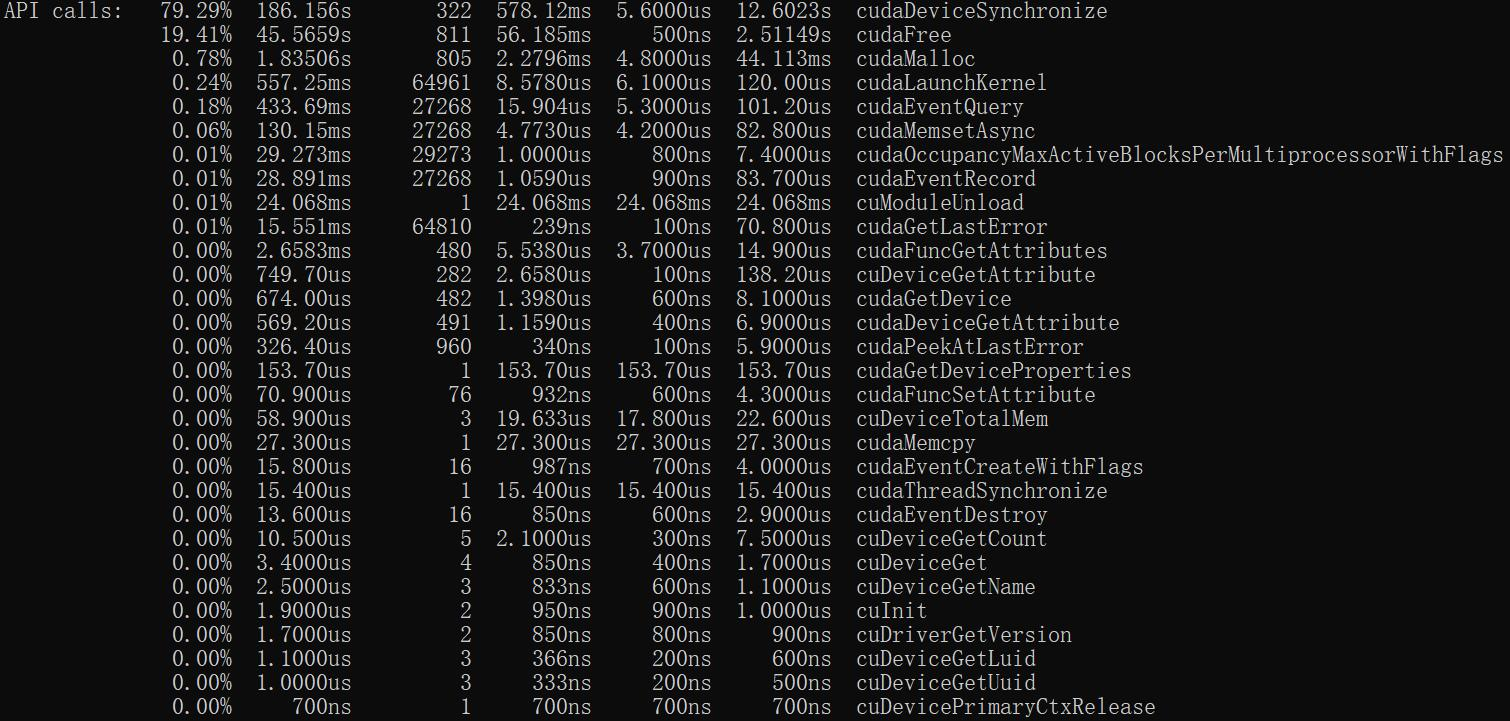
\includegraphics[width=15cm]{figures/GEMM-TF.jpg}
	\renewcommand{\thefigure}{\arabic{section}-\arabic{figure} }
	\renewcommand{\figurename}{图}
	\caption{开启张量核心下通用矩阵乘法运算的性能分析(API Calls)}
	\addtocounter{figure}{-1}
	\renewcommand{\thefigure}{\arabic{section}-\arabic{figure} }
	\renewcommand{\figurename}{Figure}
	\caption{Performance analysis of GEMM with Tensor Core On (API Calls)}
	\label{Fig.GEMMPROFTF}
\end{figure}
\begin{figure}
	\centering
	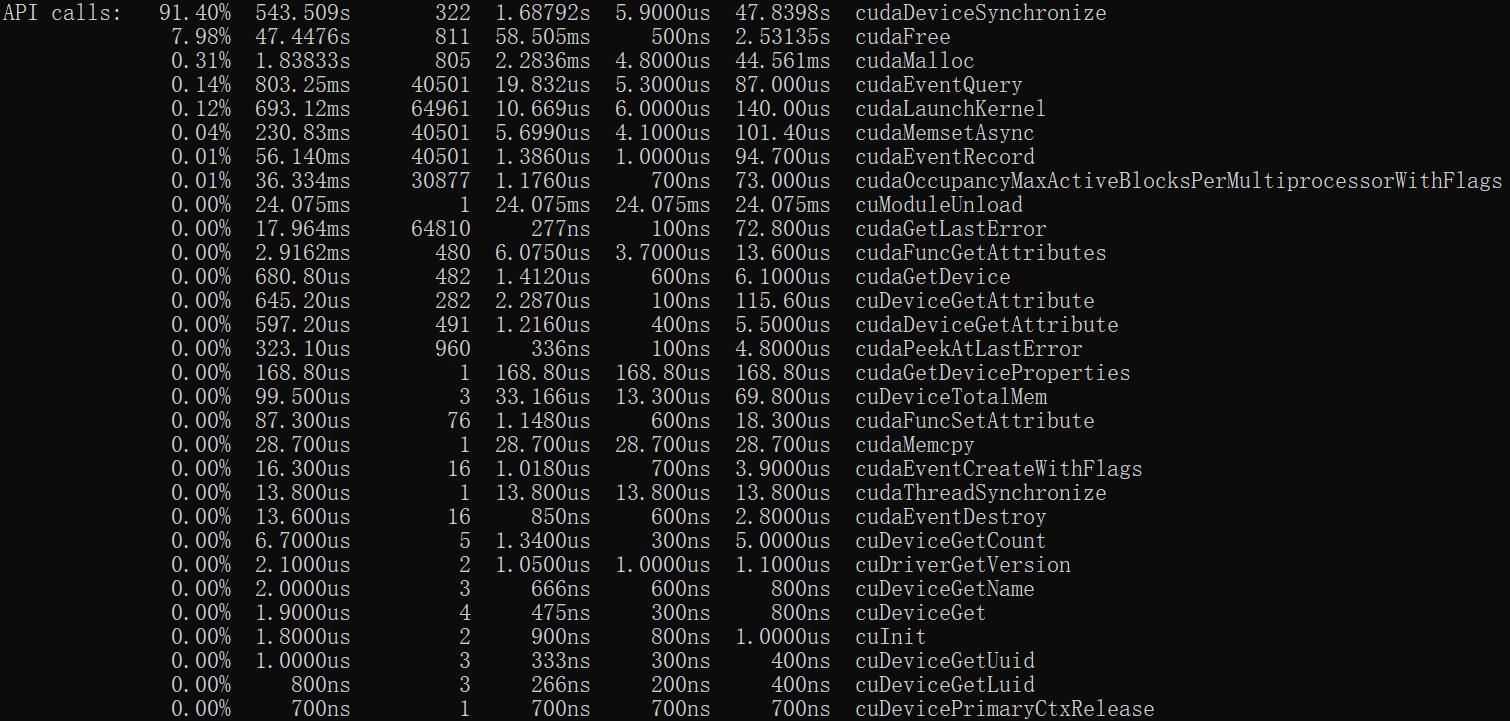
\includegraphics[width=15cm]{figures/GEMM-NOTF.jpg}
	\renewcommand{\thefigure}{\arabic{section}-\arabic{figure} }
	\renewcommand{\figurename}{图}
	\caption{关闭张量核心下通用矩阵乘法运算的性能分析(API Calls)}
	\addtocounter{figure}{-1}
	\renewcommand{\thefigure}{\arabic{section}-\arabic{figure} }
	\renewcommand{\figurename}{Figure}
	\caption{Performance analysis of GEMM with Tensor Core Off (API Calls)}
	\label{Fig.GEMMPROFNOTF}
\end{figure}
\begin{figure}
	\centering
	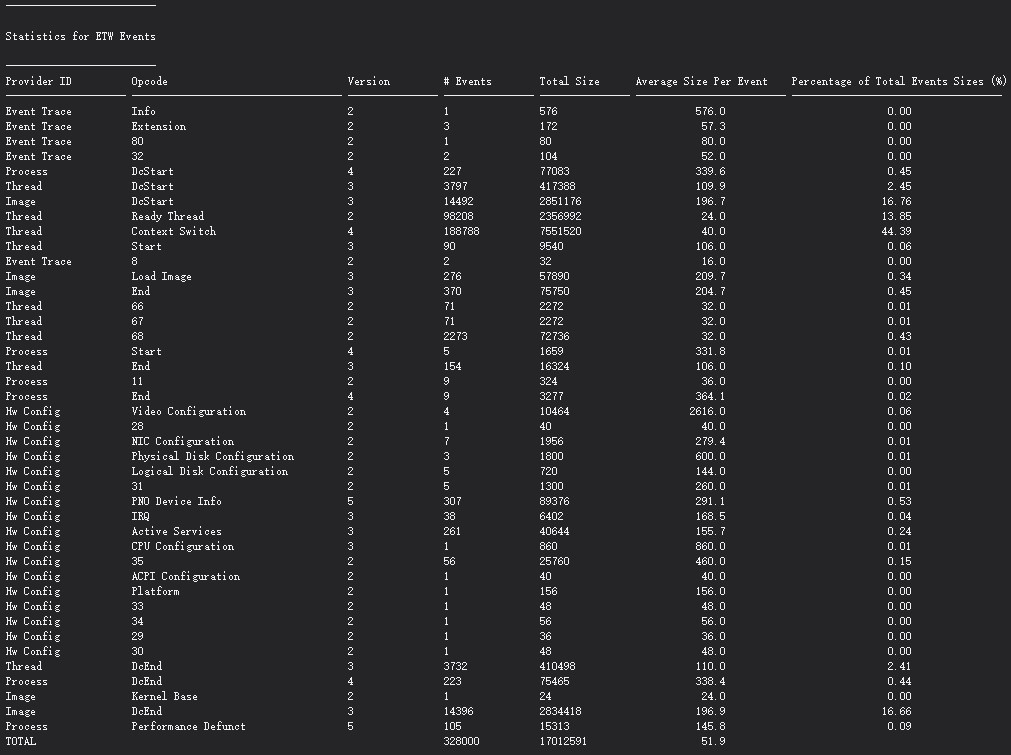
\includegraphics[width=15cm,height=10cm]{figures/GEMMSIGHTTF.jpg}
	\renewcommand{\thefigure}{\arabic{section}-\arabic{figure} }
	\renewcommand{\figurename}{图}
	\caption{开启张量核心下通用矩阵乘法运算的性能分析(上下文切换)}
	\addtocounter{figure}{-1}
	\renewcommand{\thefigure}{\arabic{section}-\arabic{figure} }
	\renewcommand{\figurename}{Figure}
	\caption{Performance analysis of GEMM with Tensor Core On (Context Switch)}
	\label{Fig.GEMMSIGHTTF}
\end{figure}
\begin{figure}
	\centering
	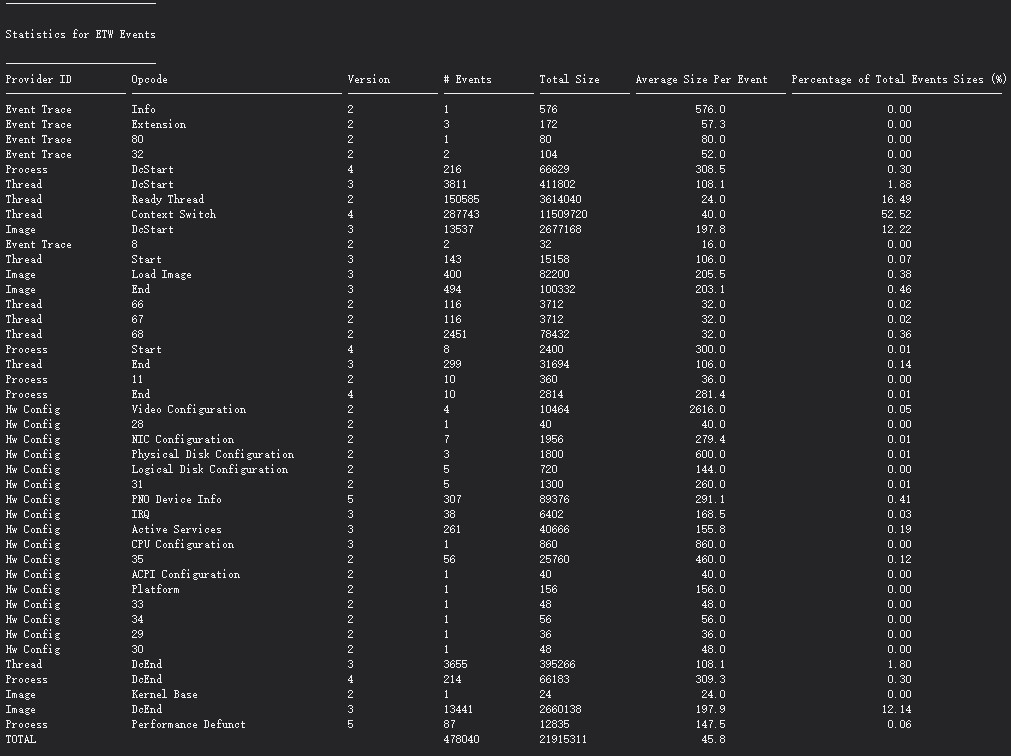
\includegraphics[width=15cm,height=10cm]{figures/GEMMSIGHTNOTF.jpg}
	\renewcommand{\thefigure}{\arabic{section}-\arabic{figure} }
	\renewcommand{\figurename}{图}
	\caption{关闭张量核心下通用矩阵乘法运算的性能分析(上下文切换)}
	\addtocounter{figure}{-1}
	\renewcommand{\thefigure}{\arabic{section}-\arabic{figure} }
	\renewcommand{\figurename}{Figure}
	\caption{Performance analysis of GEMM with Tensor Core Off (Context Switch)}
	\label{Fig.GEMMSIGHTNOTF}
\end{figure}
\begin{figure}
	\centering
	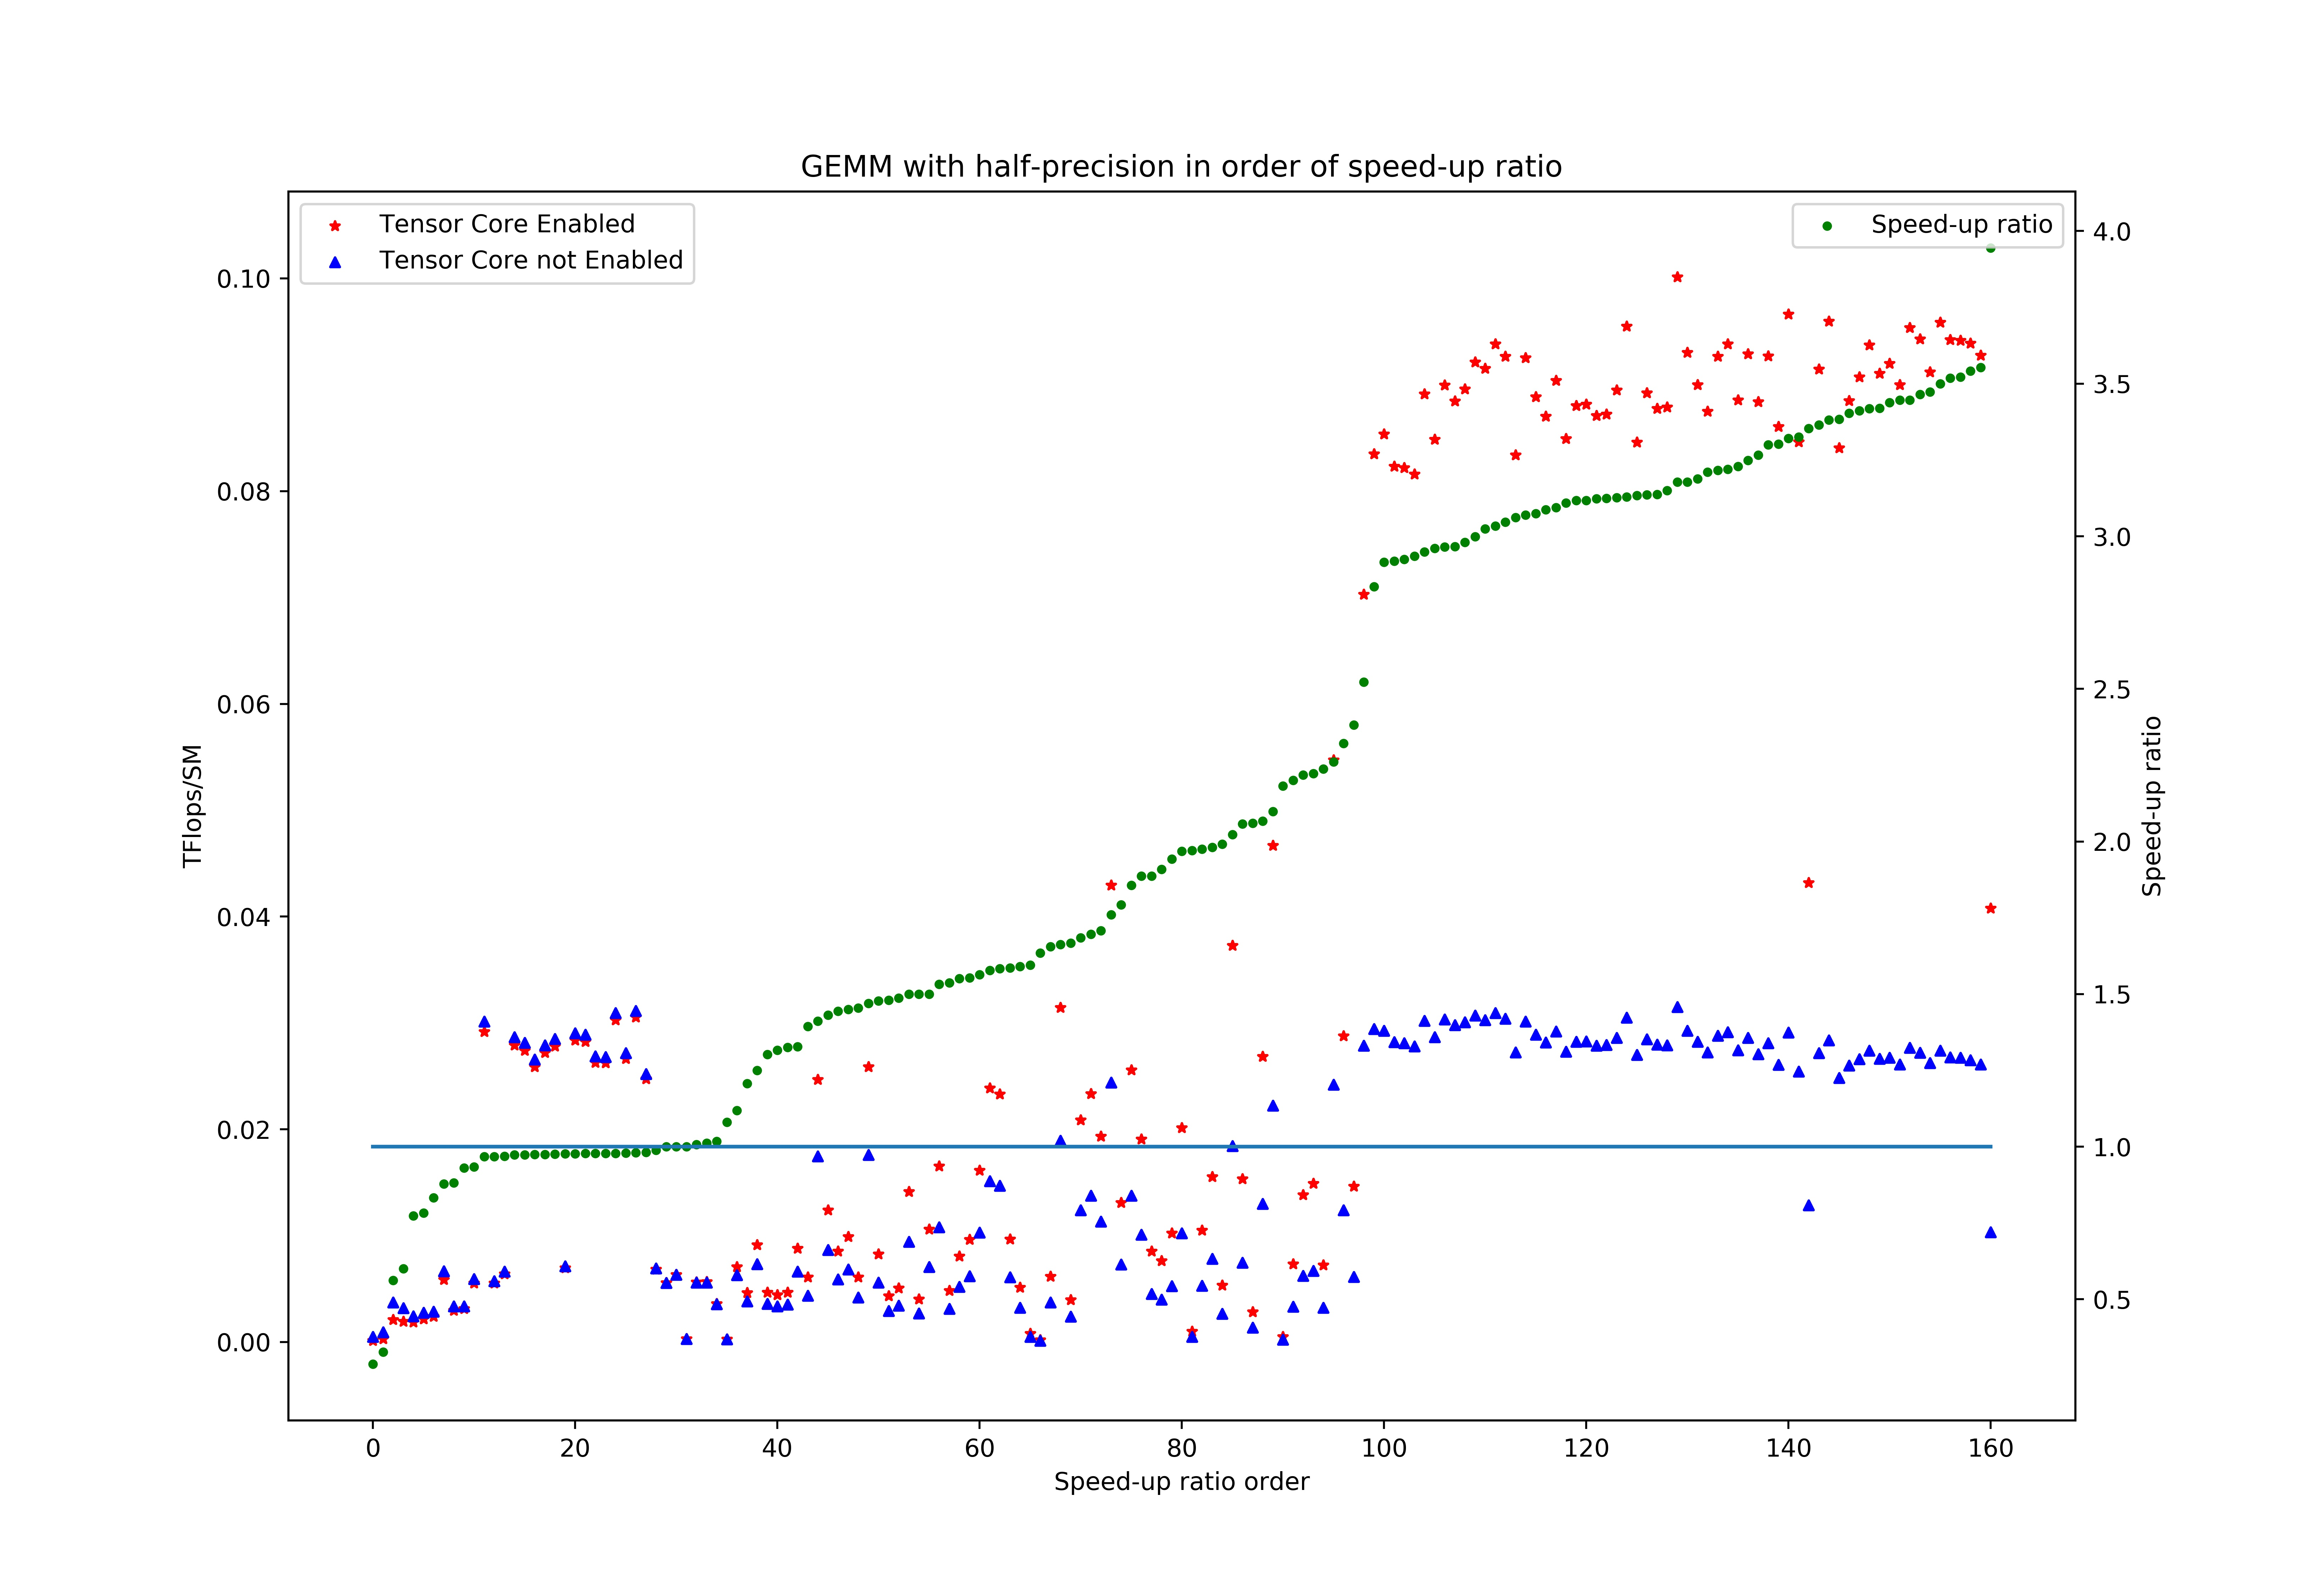
\includegraphics[width=7.5cm]{figures/GEMM-Half-TF-Byratio.jpg}
	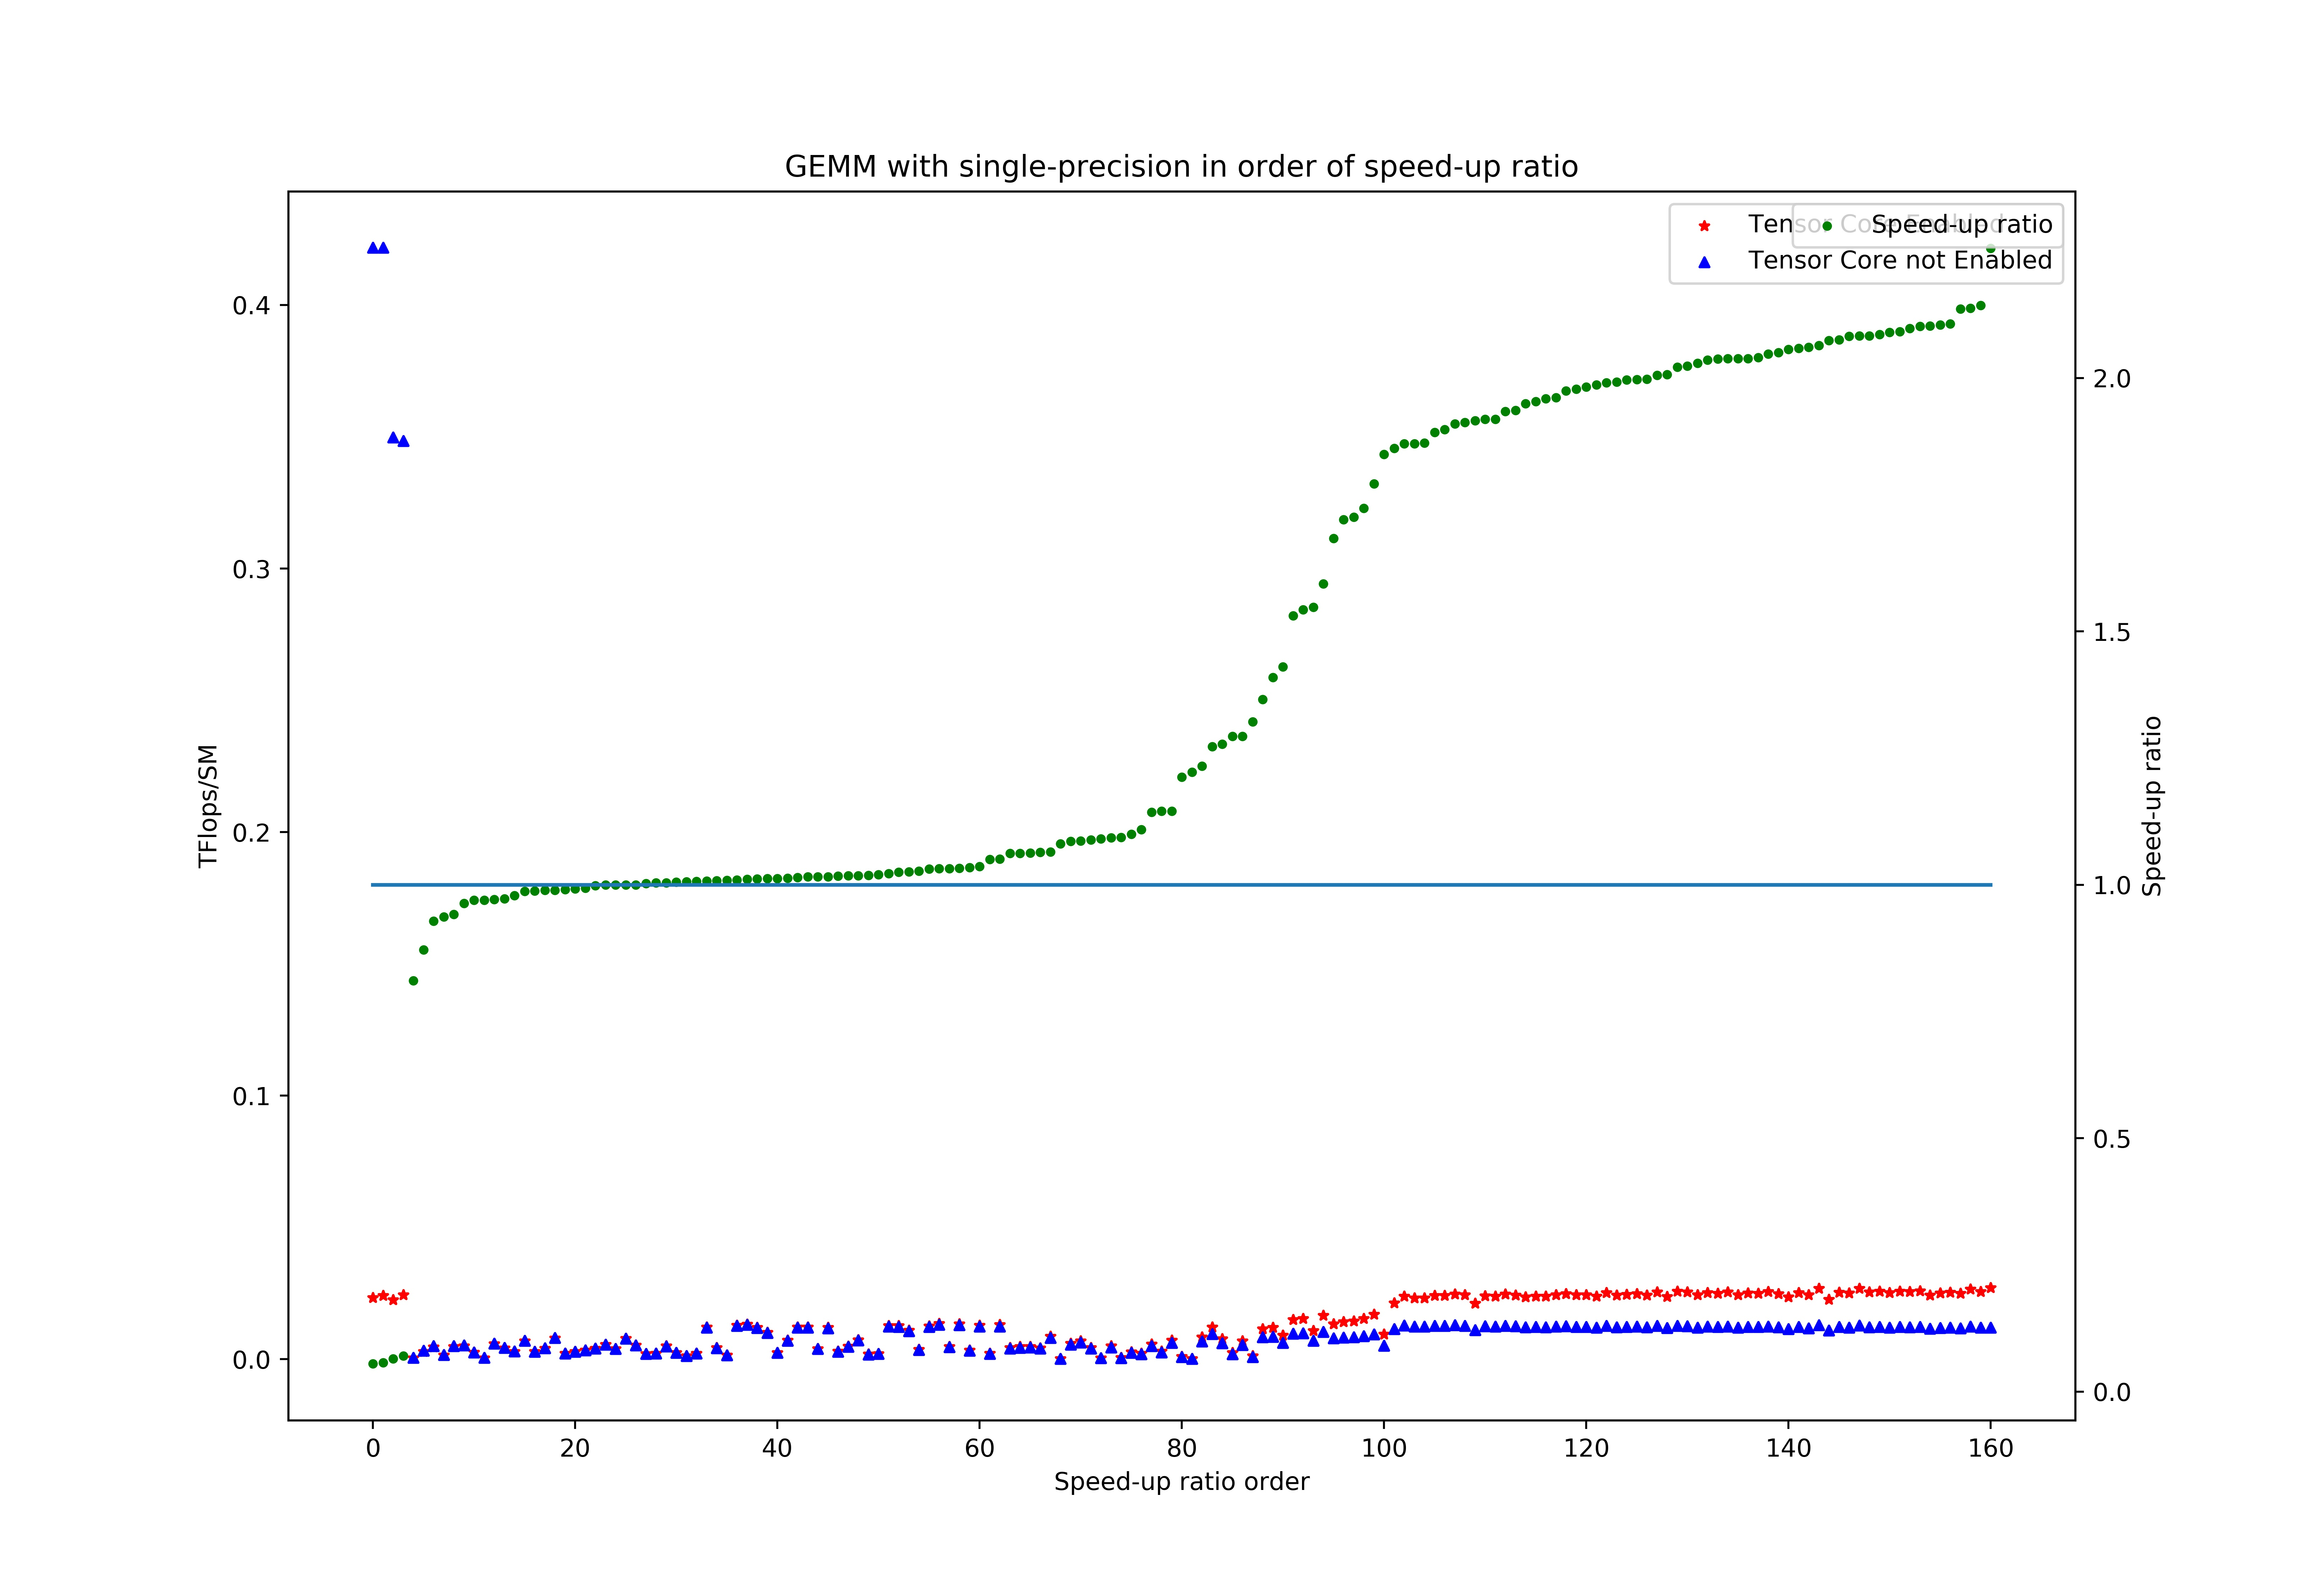
\includegraphics[width=7.5cm]{figures/GEMM-Single-TF-Byratio.jpg}
	\renewcommand{\thefigure}{\arabic{section}-\arabic{figure} }
	\renewcommand{\figurename}{图}
	\caption{半精度/单精度GEMM性能(按加速比排序)}
	\addtocounter{figure}{-1}
	\renewcommand{\thefigure}{\arabic{section}-\arabic{figure} }
	\renewcommand{\figurename}{Figure}
	\caption{Performance of GEMM at Half and Single (Sorted by speed-up ratio)}
	\label{Fig-PerfGemmByratio}
\end{figure}
\begin{figure}
	\centering
	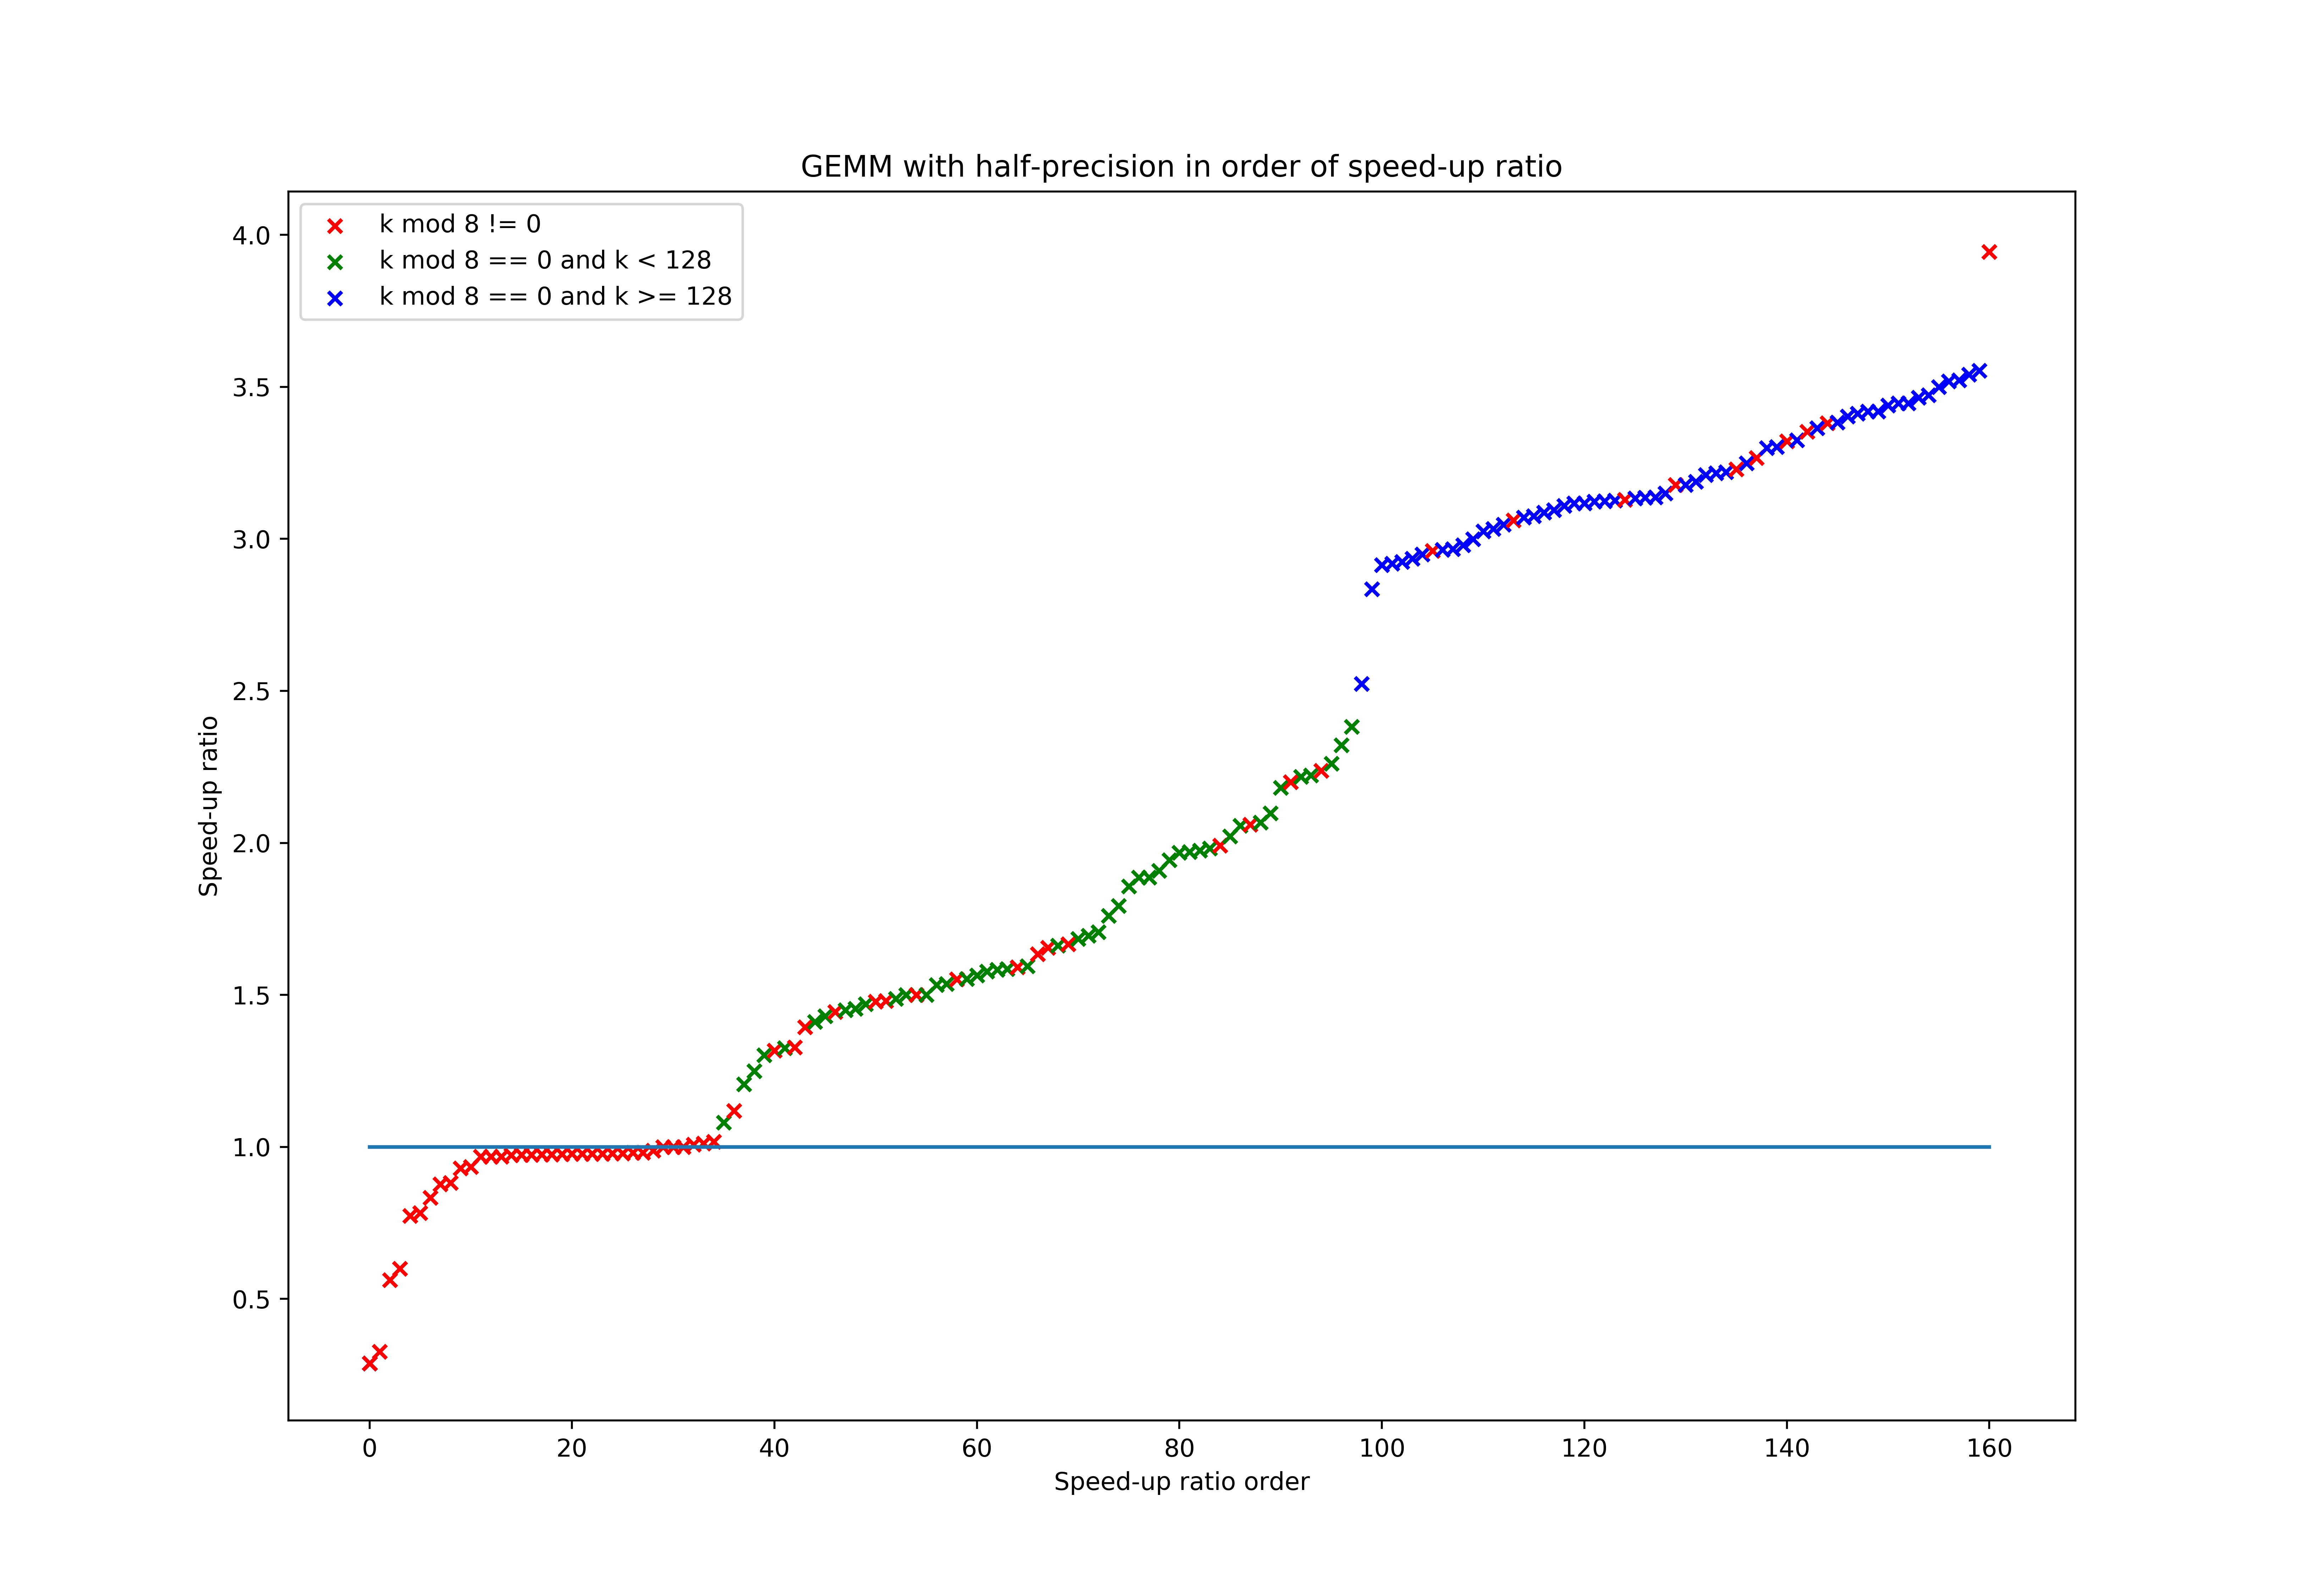
\includegraphics[width=7.5cm]{figures/GEMM-Half-TF-Byratio-Tri.jpg}
	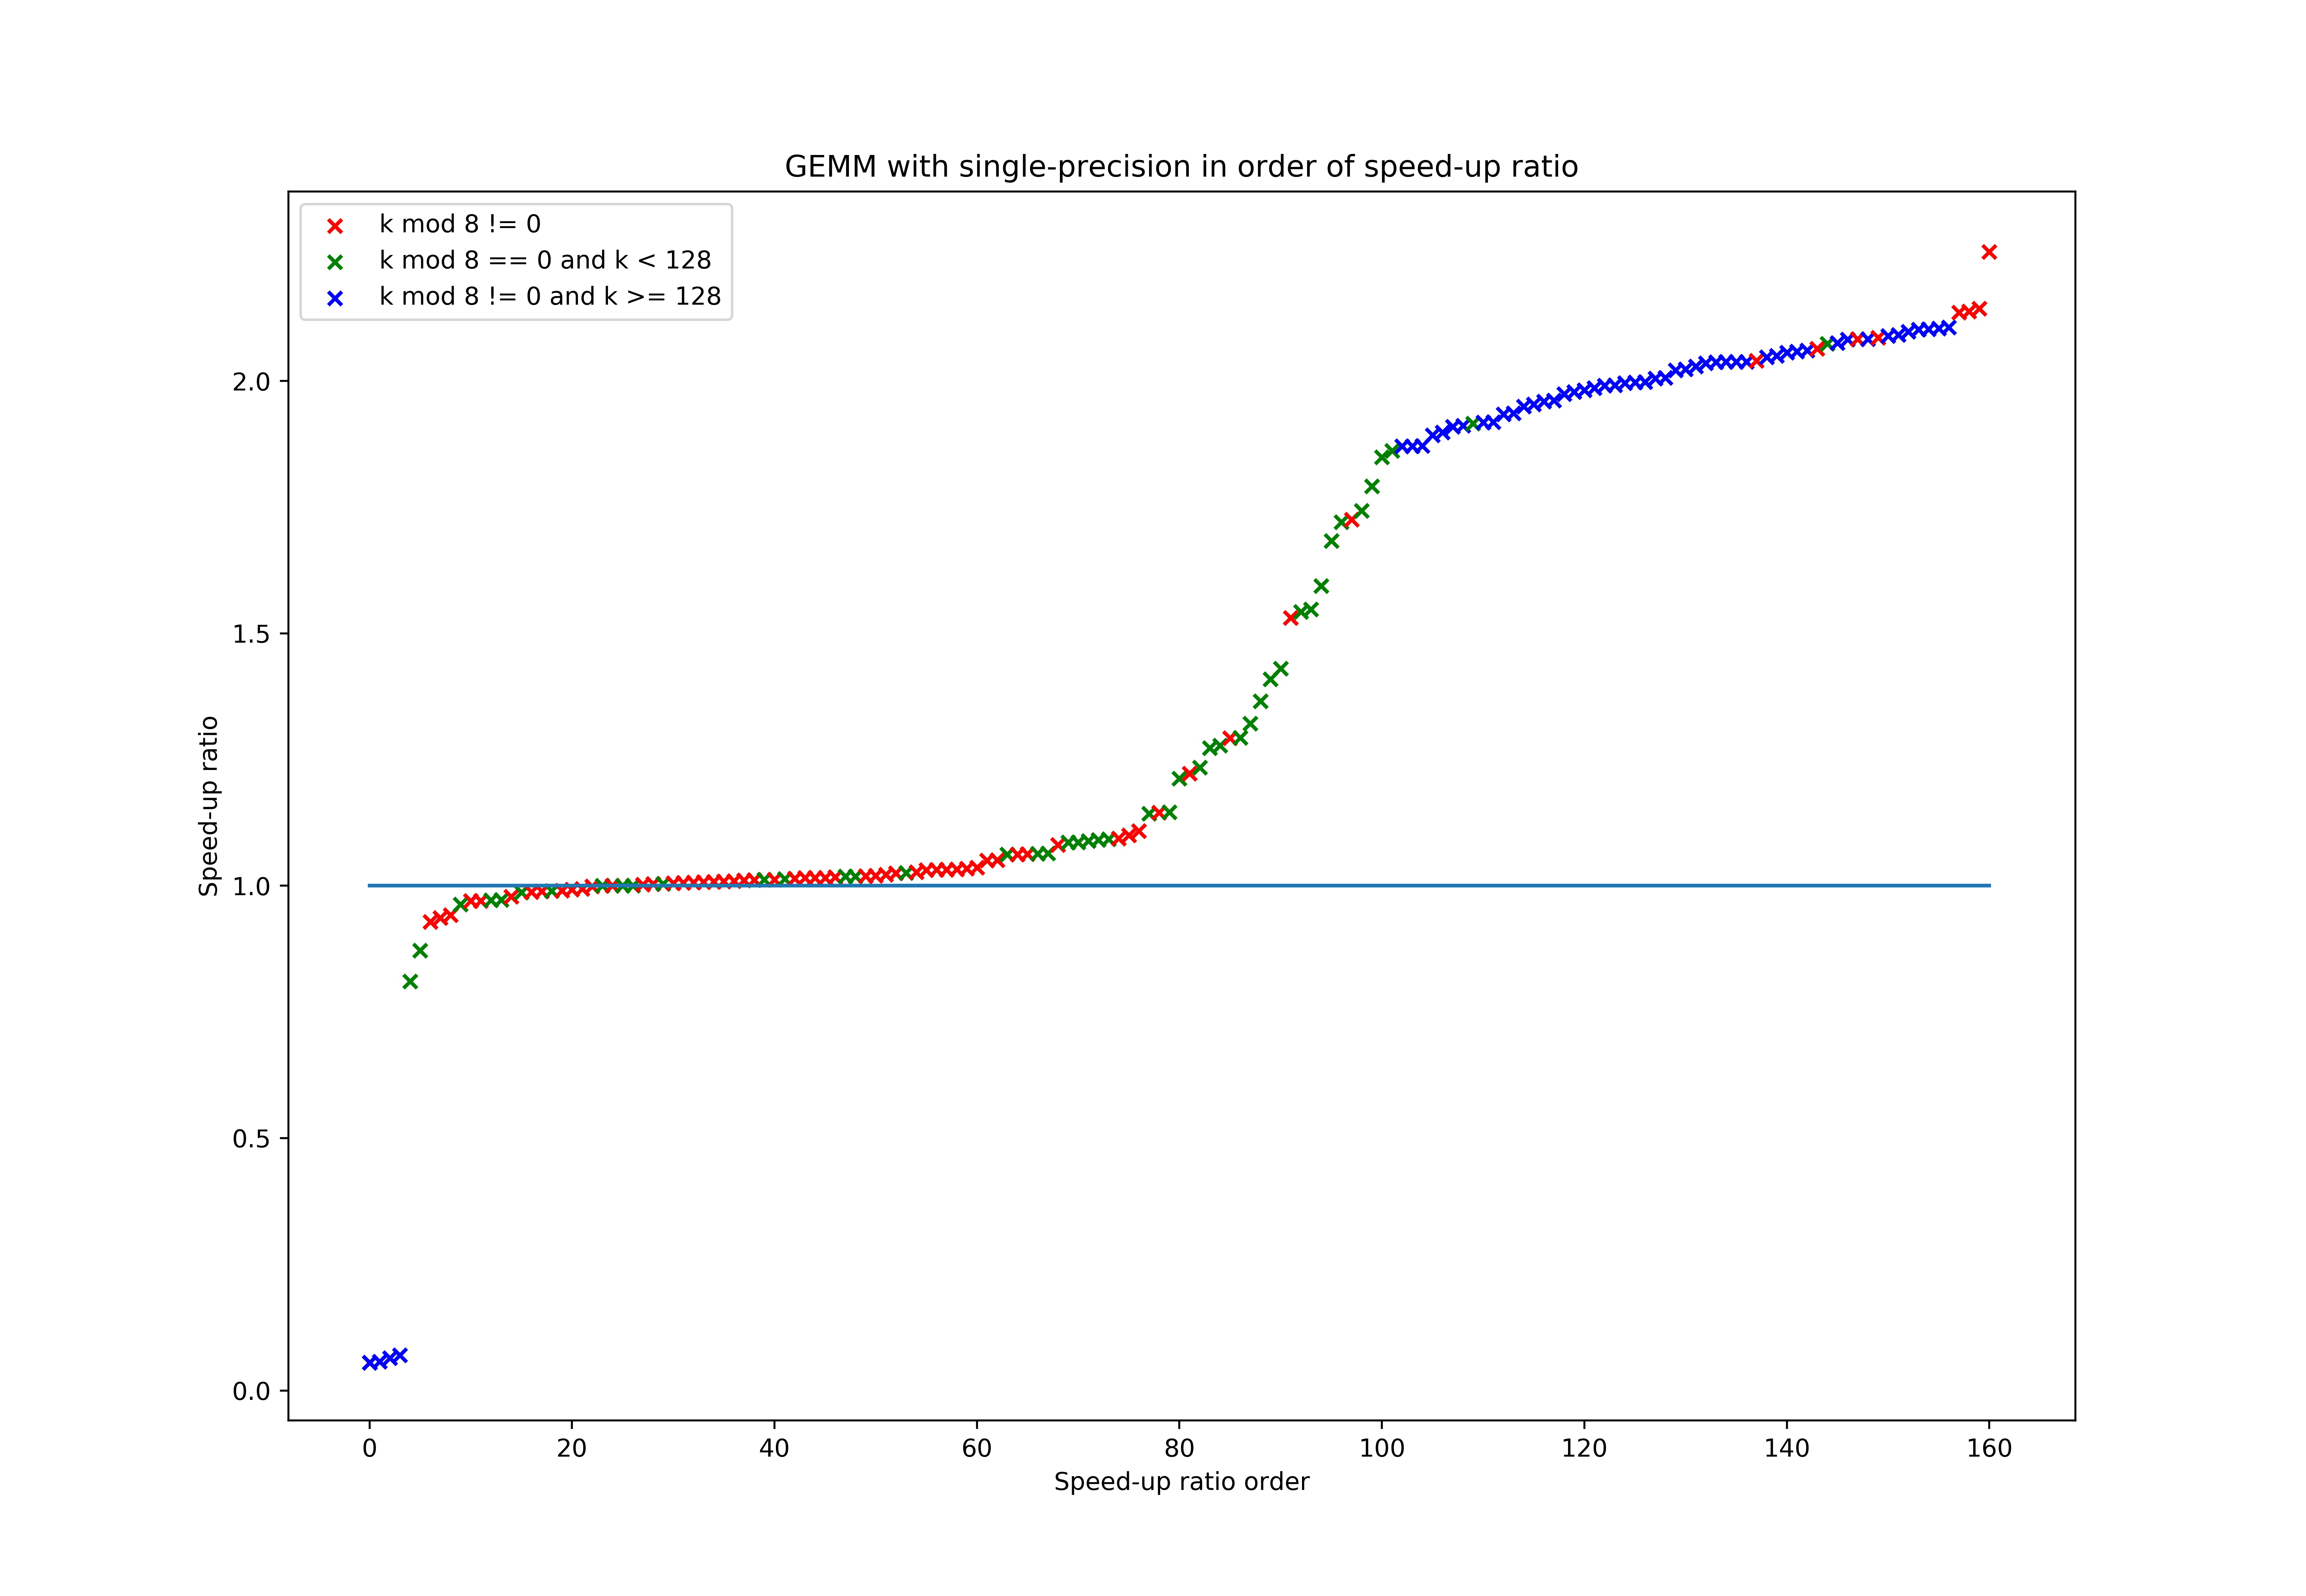
\includegraphics[width=7.5cm]{figures/GEMM-Single-TF-Byratio-Tri.jpg}
	\renewcommand{\thefigure}{\arabic{section}-\arabic{figure} }
	\renewcommand{\figurename}{图}
	\caption{半精度/单精度GEMM性能(按加速比排序,根据维度K特征着色)}
	\addtocounter{figure}{-1}
	\renewcommand{\thefigure}{\arabic{section}-\arabic{figure} }
	\renewcommand{\figurename}{Figure}
	\caption{Performance of GEMM at Half and Single (Sorted by speed-up ratio, colored with feature of K)}
	\label{Fig-PerfGemmByratioTri}
\end{figure}
\begin{figure}
	\centering
	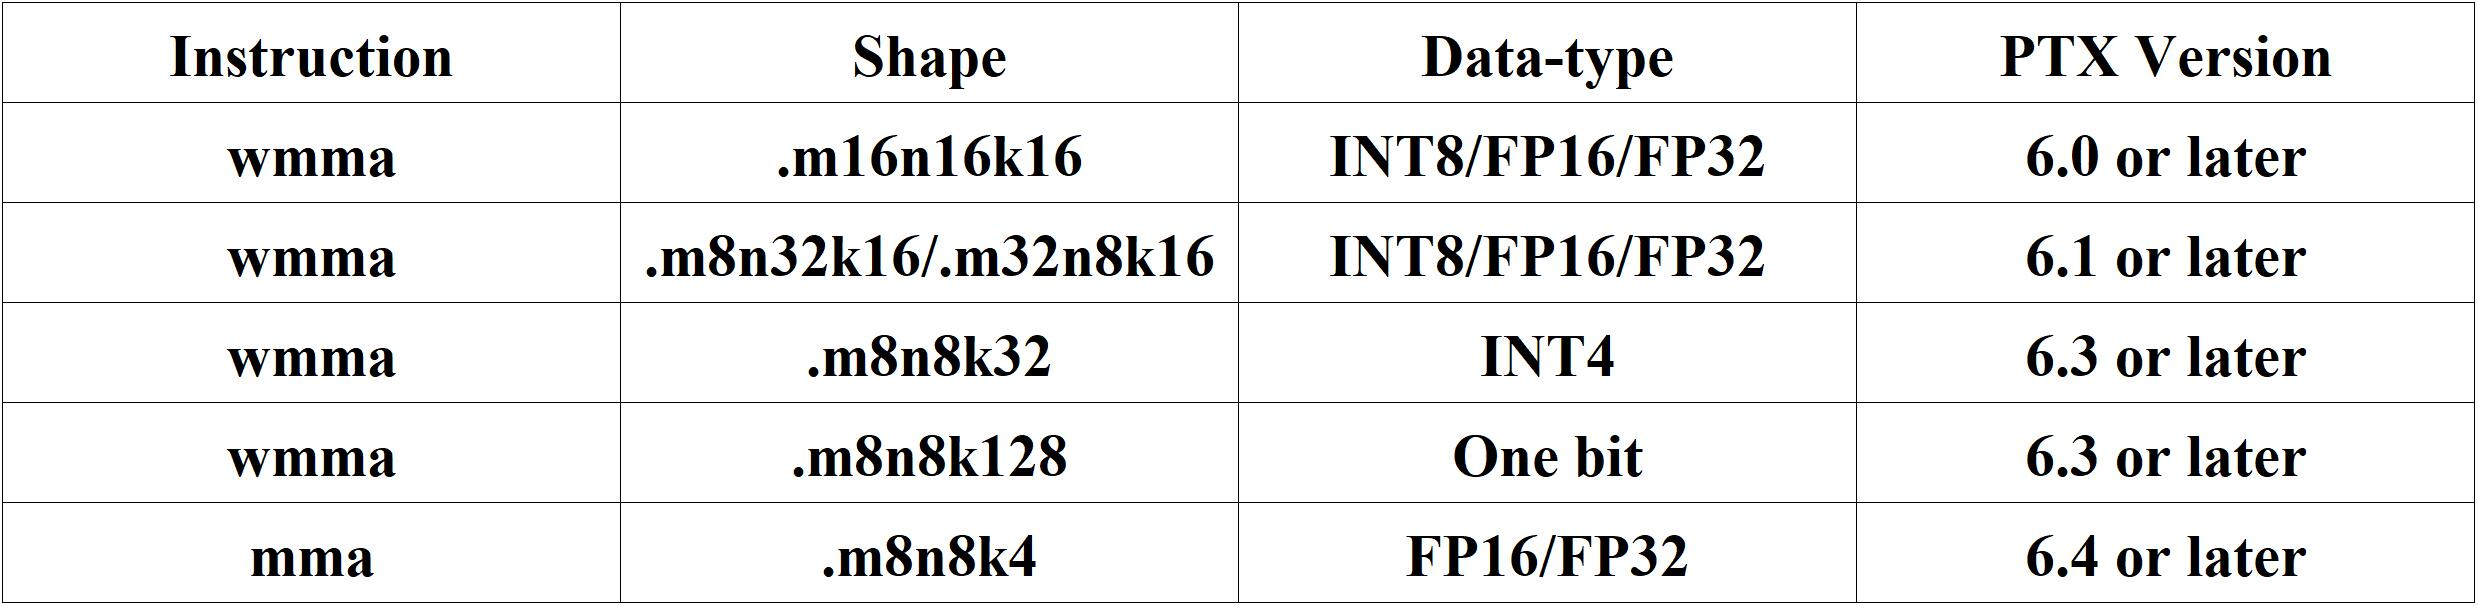
\includegraphics[width=15cm]{figures/WMMADOC.jpg}
	\renewcommand{\thefigure}{\arabic{section}-\arabic{figure} }
	\renewcommand{\figurename}{图}
	\caption{官方文档给出的wmma指令支持的分割尺寸\parencite{PTX}}
	\addtocounter{figure}{-1}
	\renewcommand{\thefigure}{\arabic{section}-\arabic{figure} }
	\renewcommand{\figurename}{Figure}
	\caption{Matrix size supported in wmma instruction based on official documentation}
	\label{Fig.WMMADOC}
\end{figure}
\begin{table}
	\centering
	\renewcommand{\thetable}{\arabic{section}-\arabic{table} }
	\renewcommand{\tablename}{表}
	\caption{GPGPU-SIM测得的各指令运行所需时钟周期}
	\addtocounter{table}{-1}
	\renewcommand{\thetable}{\arabic{section}-\arabic{table} }
	\renewcommand{\tablename}{Table}
	\caption{Clock cycle the instructions will cost based on GPGPU-SIM}
	\begin{tabular}{cc}
		\toprule
		指令	&	周期\\
		\midrule
		
		\bottomrule
	\end{tabular} \label{table-时钟周期} 
\end{table}
\paragraph{矩阵乘法运算}
\par 在新架构以矩阵乘加运算进行深度学习性能评估之前,大部分评估都采用单纯的矩阵乘法运算进行。自CUDA 6.0开始,NVIDIA推出了优化线性代数运算的cuBLAS库,而每次硬件架构更新,cuBLAS库均会针对新硬件做出改进、优化。最新的CUDA SDK 10.1则推出了cuBLASt轻量级库,在生成的应用程序大小方面做出了明显优化,性能方面则并无太多优化;由于本节旨在评估不使用张量核心的情况下,使用和不使用cuBLAS库的性能,而最新的cuBLAS库均针对张量核心进行优化,故本节中使用的cuBLAS库是基于CUDA SDK 8.0。本节将考察使用和不使用CUDA SDK 8.0中的cuBLAS库的情况下使用GPU进行矩阵乘法运算的性能。
\subparagraph{实验结果}
\par 图\ref{Fig.CUBLASPerf}显示了使用和不使用CUDA SDK 8.0中cuBLAS库进行矩阵乘法运算的性能。随着数据规模的增长,基于cuBLAS库的应用的单精度浮点矩阵乘法运算性能稳定在13TFlops左右;而不适用cuBLAS库的应用尽管不明显,其单精度浮点矩阵运算性能仍随着数据规模的增长而增长,最终稳定在0.13TFlops左右。实验中使用的数据集并未如上一节中测试张量核心时的数据,分为能否被8整除,而是全部随机。实验结果发现在张量核心以及相关指令尚未出现时,使用cuBLAS库时矩阵形状并不会对性能造成显著影响。
\begin{figure}
	\centering
	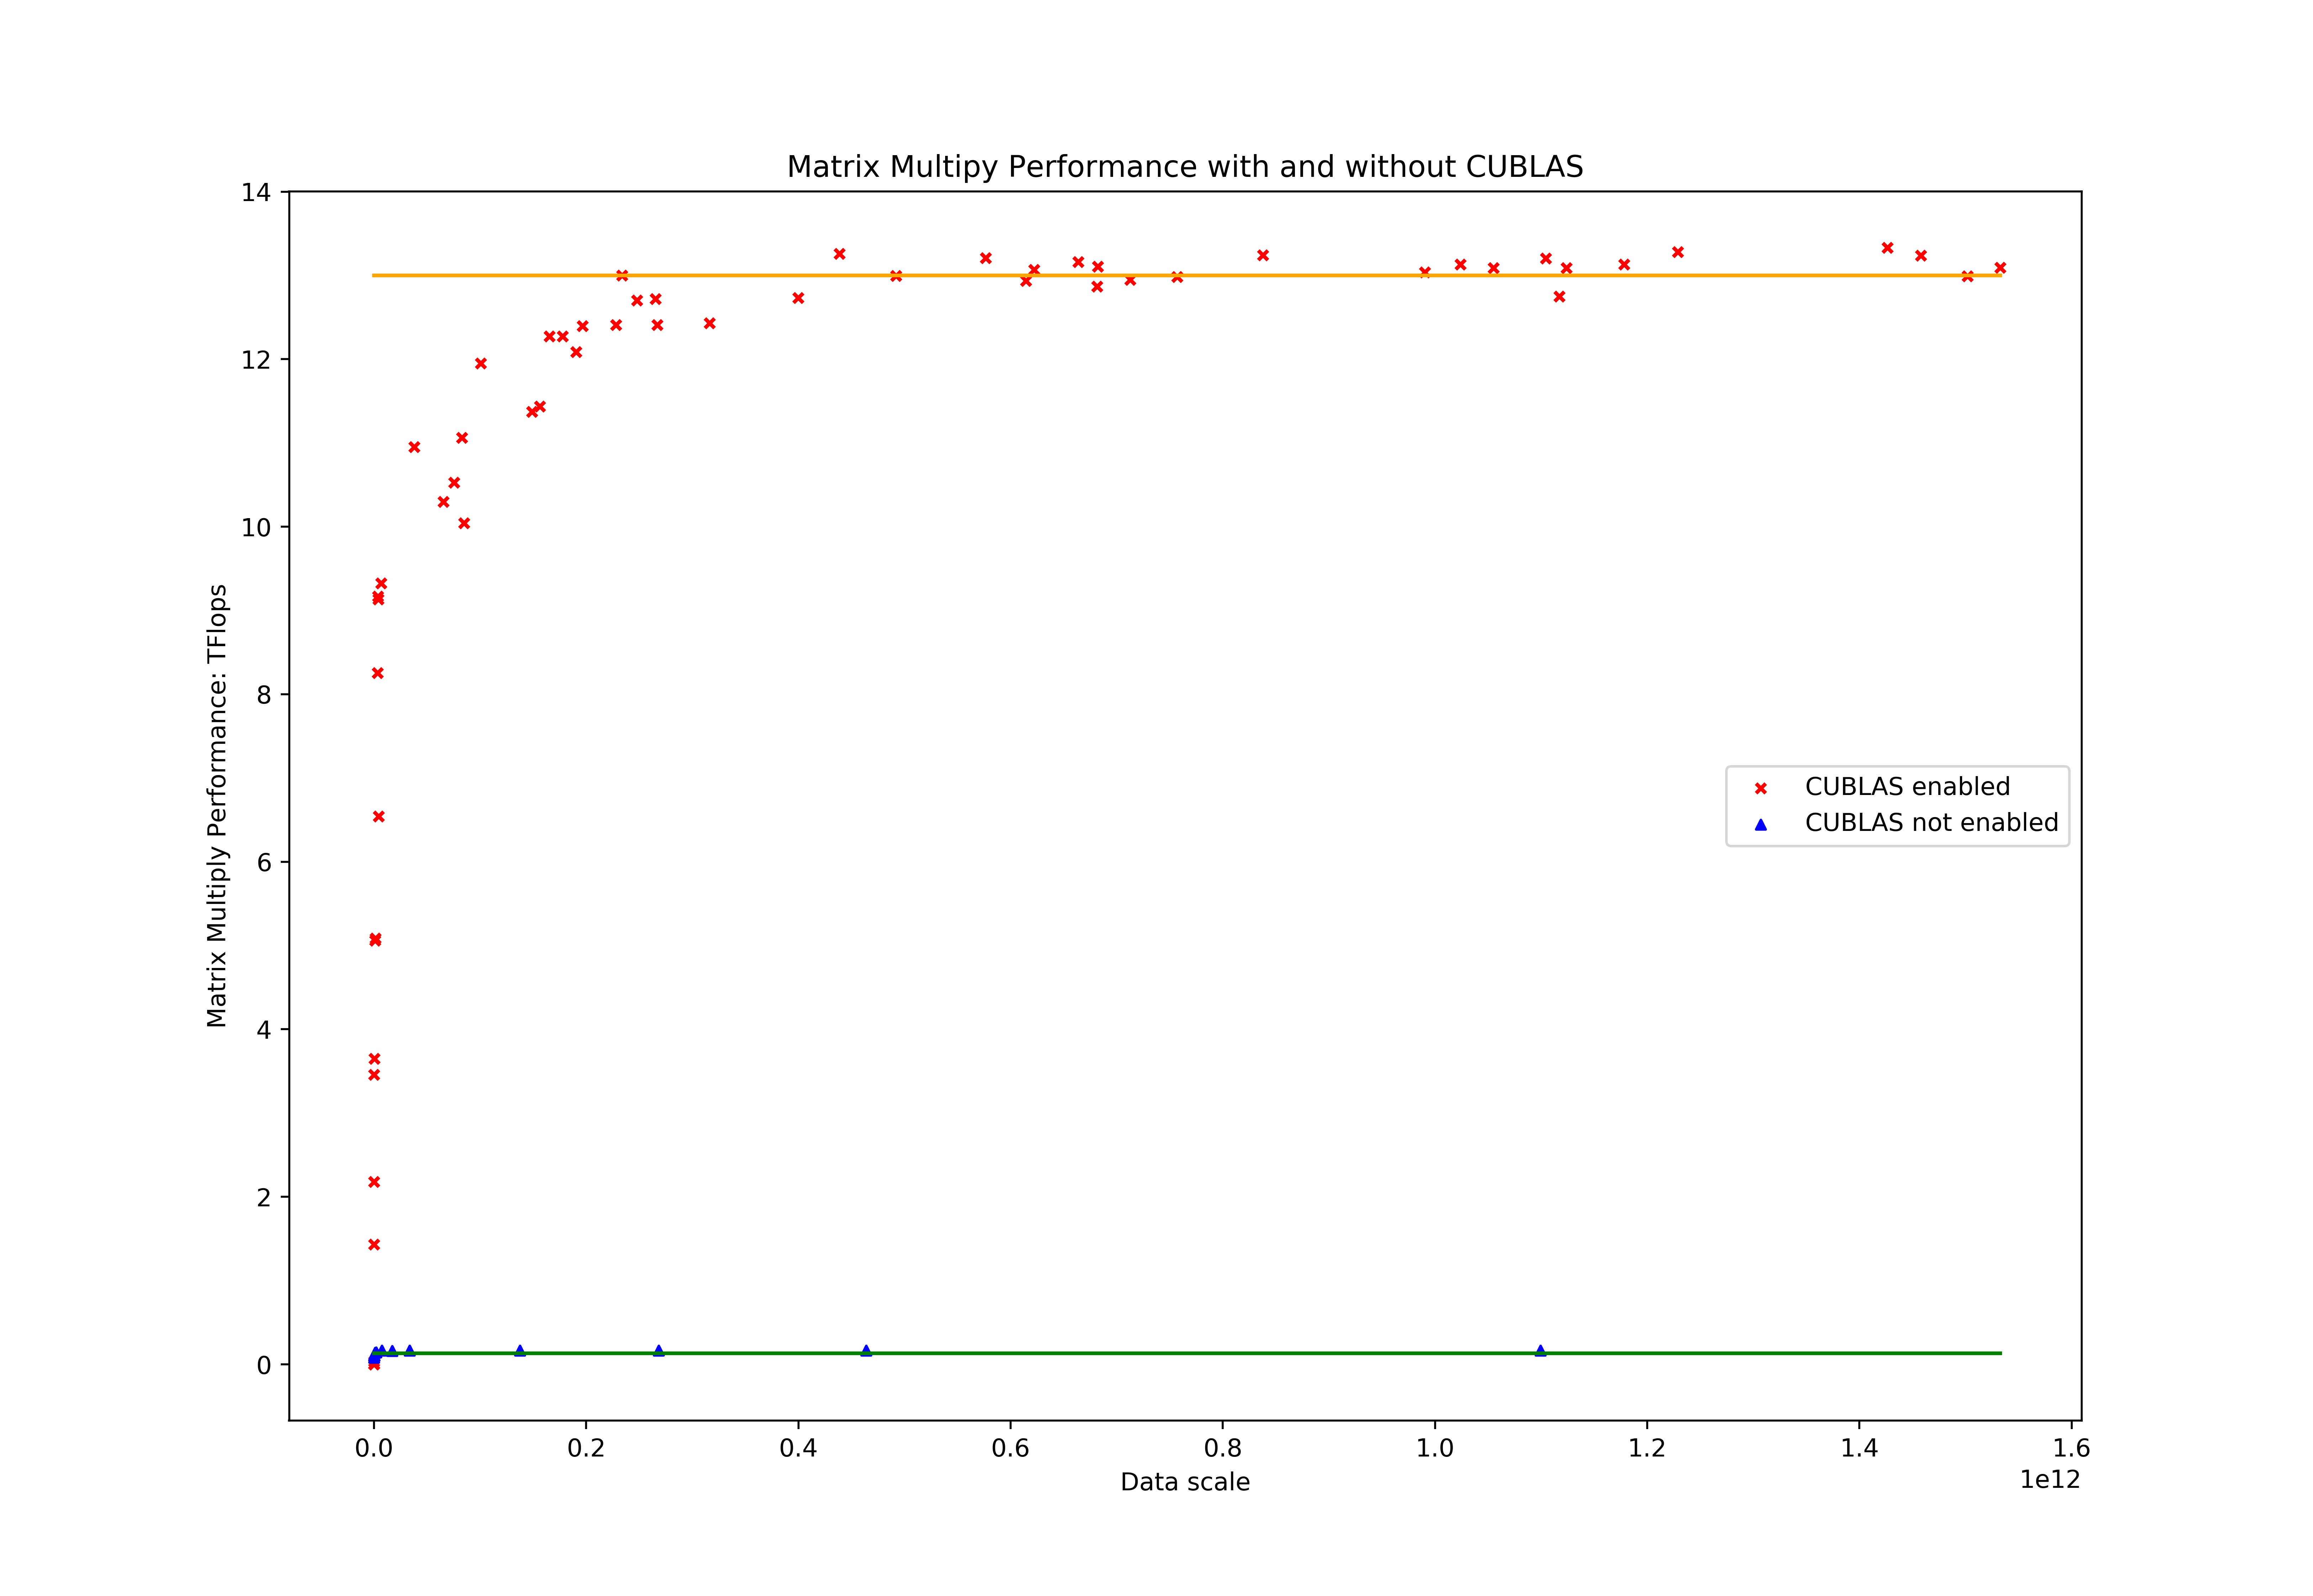
\includegraphics[width=15cm]{figures/CUBLASPerf.jpg}
	\renewcommand{\thefigure}{\arabic{section}-\arabic{figure} }
	\renewcommand{\figurename}{图}
	\caption{使用和不使用cuBLAS库时的矩阵乘法运算性能}
	\addtocounter{figure}{-1}
	\renewcommand{\thefigure}{\arabic{section}-\arabic{figure} }
	\renewcommand{\figurename}{Figure}
	\caption{Performance of Matrix Multiply with and without cuBLAS library}
	\label{Fig.CUBLASPerf}
\end{figure}
\subparagraph{结果分析}
\par 需要注意的是,在实验中不使用cuBLAS库的矩阵乘法是基于GPU直接进行数值计算的,性能较差的同时支持的数据量也不够理想(因系统、硬件和驱动的原因,CUDA程序的一个内核在Windows 10操作系统下运行超过一定时间即会抛出超时异常,而不使用cuBLAS、采用直接计算的方法计算矩阵乘积速度较慢,导致大数据量下程序超时)。且由于内存分配模式的原因,在直接计算中,无法被32整除的维数需要被填充为32的倍数,在某些情况下会造成大量的内存浪费。故考虑到性能、程序健壮性等因素,在不支持张量核心的设备上进行矩阵乘法运算应尽可能使用cuBLAS库。

\paragraph{卷积运算}
\par 在深度学习中,卷积作为提取特征、过滤图像噪声的一种方式,无疑是从业者最为熟悉、存在于最多应用中的计算。且在图像处理中,卷积运算也是非常重要的一环。计算卷积有若干方法,本节将使用NVIDIA官方发布的Benchmark样例评估这些不同方法在不同情况下的性能。当然,由于还存在解卷积运算,故精度也在本实验考虑范围之内,以满足不同任对队速度和精度的取舍。
\subparagraph{实验结果}
\par 本节的实验涉及如下几种卷积计算方法:基于快速傅里叶变换的卷积;基于通用矩阵乘法的卷积和基于传统的直接计算的卷积(cudnn中将这一方法命名为Conv\_Direct),即分别计算输出图像每一个单元的值。而这三种方法在CUDA的实现中也有差异,如表\ref{table-CONV}所示。
\begin{table}
	\centering
	\renewcommand{\thetable}{\arabic{section}-\arabic{table} }
	\renewcommand{\tablename}{表}
	\caption{实验中的几种卷积计算方式}
	\addtocounter{table}{-1}
	\renewcommand{\thetable}{\arabic{section}-\arabic{table} }
	\renewcommand{\tablename}{Table}
	\caption{Methods to calculate convolution}
	\begin{tabular}{cc}
		\toprule
		卷积计算方式	&	描述\\
		\midrule
		基于快速傅里叶变换(FFT)的CUDA内建的卷积 & 使用CUDA提供的基于FFT的卷积库\\
		基于快速傅里叶变换(FFT)的自定义卷积 & 使用CUDA提供的FFT库实现卷积\\
		基于通用矩阵乘法(GEMM)的CUDA内建的卷积 & 使用CUDA提供的利用张量核心的API\\
		直接卷积(全局内存,Global Memory) & 直接计算每一个单元的值,基于全局内存\\
		直接卷积(纹理内存,Texture Memory) & 直接计算每一个单元的值,基于纹理内存\\
		\bottomrule
	\end{tabular} \label{table-CONV} 
\end{table}
\par 其中,访问纹理内存时使用传统的OpenCL/GL中的实现方式。因纹理内存的访存、缓存方式与一般存储系统不同,在测试时分为行卷积和咧卷积。实验中卷积核步进、图像填充(padding)均不变,性能采用兆像素每秒(MPix/s)计算。
\begin{figure}
	\centering
	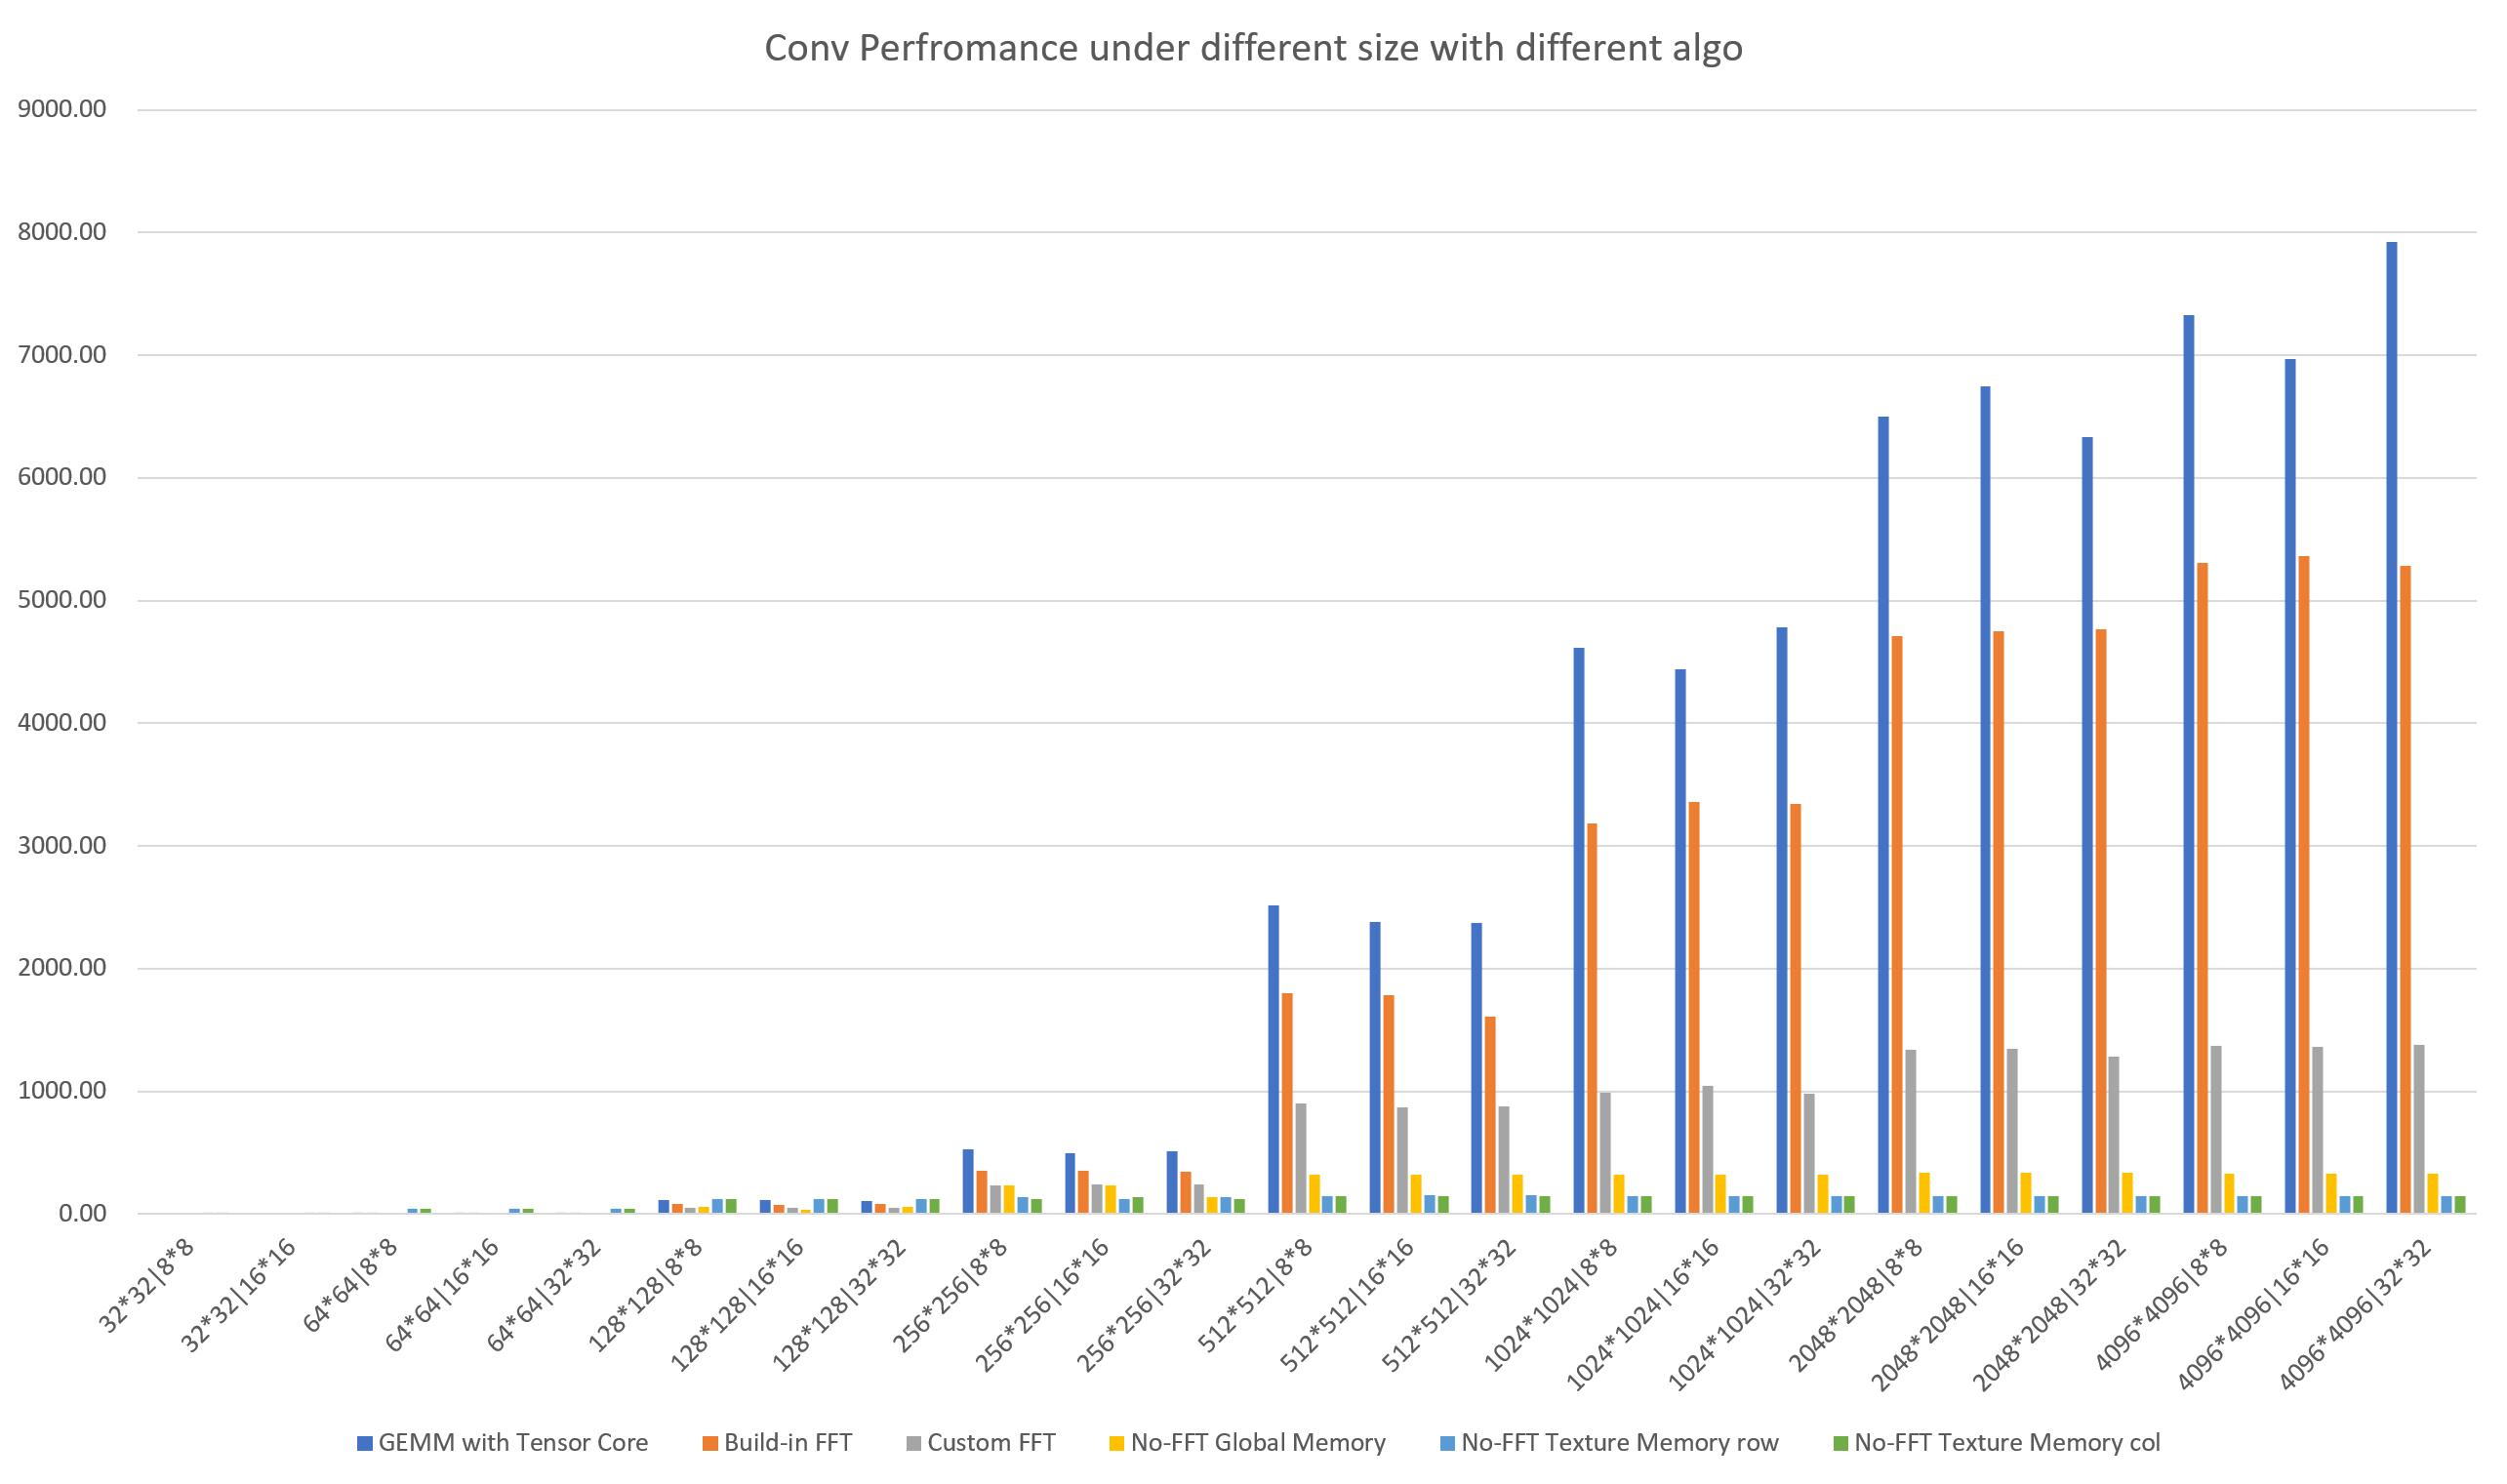
\includegraphics[width=15cm]{figures/CONVPerf.jpg}
	\renewcommand{\thefigure}{\arabic{section}-\arabic{figure} }
	\renewcommand{\figurename}{图}
	\caption{使用不同计算方法的卷积性能}
	\addtocounter{figure}{-1}
	\renewcommand{\thefigure}{\arabic{section}-\arabic{figure} }
	\renewcommand{\figurename}{Figure}
	\caption{Performance of convolution based on different algorithm}
	\label{Fig.CONVPerf}
\end{figure}
\subparagraph{结果分析}
\paragraph{神经网络推理}
\subparagraph{实验结果}
\subparagraph{结果分析}
\subsubsection{基于CUDA源码的应用}
\paragraph{卷积神经网络}
\subparagraph{实验结果}
\subparagraph{结果分析}
\paragraph{并行支持向量机}
\subparagraph{实验结果}
\subparagraph{结果分析}
\subsubsection{基于TensorFlow框架的应用}
\subparagraph{实验结果}
\subparagraph{结果分析}